% !TeX program = xelatex
% Compile from the DSA5101 folder: latexmk -xelatex DSA5101_Cheatsheet.tex
% Questions are vector excerpts from the five course PDFs, grouped by topic.
\documentclass[10pt,a4paper]{article}
\usepackage[a4paper,landscape,left=10mm,right=10mm,top=9mm,bottom=11mm,nohead,footskip=6mm]{geometry}
\usepackage{amsmath}
\usepackage{fontspec,unicode-math}
\setmainfont{STIXTwoText}[Extension=.otf,UprightFont=*-Regular,BoldFont=*-Bold,ItalicFont=*-Italic,BoldItalicFont=*-BoldItalic]
\setmathfont{STIXTwoMath-Regular.otf}
\usepackage{graphicx,enumitem,multicol,titlesec,needspace}
\usepackage[protrusion=true,expansion=false]{microtype}
\usepackage[unicode,hidelinks,bookmarksopen,bookmarksdepth=2]{hyperref}
\usepackage{bookmark,booktabs,tikz}
\usetikzlibrary{arrows.meta,shapes.misc}

\hypersetup{pdftitle={DSA5101 - Exam Cheatsheet}}
\pagestyle{plain}
\setlength{\parindent}{0pt}
\setlength{\parskip}{3.5pt}
\setlength{\columnsep}{9mm}
\setlength{\emergencystretch}{2em}

\setlist{nosep,leftmargin=1.25em}
\newcommand{\tightlist}{}
\setcounter{secnumdepth}{0}
\raggedbottom

\newcommand{\headingfont}{\fontsize{12pt}{14pt}\selectfont\bfseries}
\newcommand{\algorithmfont}{\fontsize{11pt}{13pt}\selectfont\bfseries}
\newcommand{\lectureband}[1]{%
  \begingroup
  \setlength{\fboxsep}{4pt}%
  \colorbox{black!8}{%
    \parbox{\dimexpr\linewidth-2\fboxsep\relax}{\raggedright\strut#1\strut}}%
  \endgroup}
\titleformat{\section}[block]{\headingfont}{}{0pt}{\lectureband}
\titleformat{\subsection}[block]{\algorithmfont\raggedright}{}{0pt}{%
  \rule[-.2ex]{1pt}{1.35ex}\hspace{5pt}}
\titlespacing*{\section}{0pt}{10pt}{4pt}
\titlespacing*{\subsection}{0pt}{9pt}{2pt}


\makeatletter
\newcommand{\maptag}[1]{\phantomsection\@bsphack\protected@write\@auxout{}{\string\newlabel{#1}{{}{\thepage}{}{\@currentHref}{}}}\@esphack}
\makeatother
\newcommand{\lecture}[2]{%
  \par\needspace{48pt}%
  \section{L#1. #2}\label{lecture:#1}}
\newcommand{\topic}[2]{\subsection{#2}\label{topic:#1}}
\newcommand{\key}[1]{#1:\enspace}
\newcommand{\literal}[1]{“#1”}
\newcommand{\steps}[1]{\begin{enumerate}[label=\arabic*.,leftmargin=1.5em,itemsep=1pt,topsep=2pt]#1\end{enumerate}}
\newcommand{\outline}[2]{\hyperref[lecture:#1]{\makebox[2.3em][l]{L#1}#2\hfill\pageref*{lecture:#1}}\par}

\newcommand{\blocklabel}[1]{\par\noindent#1\par\nobreak}
\newcommand{\answer}[1]{%
  \par\addvspace{4pt}%
  \blocklabel{#1Hướng dẫn giải}}
\newcommand{\guidepart}[1]{#1\enspace}
\newlist{guidesteps}{enumerate}{1}
\setlist[guidesteps]{label=\arabic*.,leftmargin=1.65em,topsep=0pt,
  itemsep=1pt,parsep=0pt,partopsep=0pt}
\NewDocumentCommand{\ask}{o m m m}{%
  \par\addvspace{7pt}%
  \blocklabel{\maptag{question:#2}\IfValueT{#1}{\maptag{question:#1}}%
    \rule[.55ex]{14pt}{.4pt}\enspace Câu hỏi: #3%
    \if\relax\detokenize{#4}\relax\else\hfill #4\fi}}
\newcommand{\original}[3]{%
  \par\noindent\includegraphics[page=#2,viewport=#3,clip,width=\linewidth]{#1}\par}
\newcommand{\qlink}[2]{\hyperref[question:#1]{#2}}
\newcommand{\hard}[2]{%
  \par\addvspace{5pt}%
  \blocklabel{Dạng khó: #2\enspace\qlink{#1}{[Đề]}}}

\newenvironment{example}[2]{%
  \par\addvspace{6pt}\noindent\begin{minipage}{\linewidth}%
  \setlength{\parskip}{3.5pt}%
  \setlength{\abovedisplayskip}{4pt}\setlength{\belowdisplayskip}{4pt}%
  \raggedright
  \blocklabel{Ví dụ: \qlink{#1}{#2}}%
}{\par\end{minipage}\par\addvspace{4pt}}
\newenvironment{examtable}[1]{%
  \par\addvspace{3pt}\noindent\hbox to \linewidth\bgroup\hfil
  \setlength{\tabcolsep}{4pt}%
  \renewcommand{\arraystretch}{1.12}\begin{tabular}{#1}%
}{\end{tabular}\hfil\egroup\par\addvspace{3pt}}
\newenvironment{diagram}{%
  \par\addvspace{3pt}\noindent\hbox to \linewidth\bgroup\hfil
}{\hfil\egroup\par\addvspace{3pt}}

\AtBeginDocument{\raggedright\allowdisplaybreaks[1]}

\begin{document}
\begin{multicols}{2}
\raggedcolumns
\pdfbookmark[0]{Mục lục chủ đề}{index-bookmark}
{\headingfont DSA5101 Cheatsheet}\par
\blocklabel{Mục lục chủ đề}
{\setlength{\parskip}{1.5pt}
\outline{1}{Frequent itemsets \& association rules}
\outline{2}{Similar items \& locality-sensitive hashing}
\outline{3}{Clustering}
\outline{4}{Dimensionality reduction}
\outline{5}{Recommender systems}
\outline{6}{Link analysis \& graph ranking}
\outline{7}{Communities \& graph embeddings}
\outline{8}{Data streams}
\outline{9}{Online matching, BALANCE \& bandits}
\outline{10}{Submodular optimization}
}

\lecture{1}{Frequent itemsets \& association rules}

\topic{bonferroni}{Bonferroni's Principle (multiple comparisons)}
\key{Khi dùng} Đề thử rất nhiều mẫu rồi hỏi có bao nhiêu phát hiện chỉ do tình cờ.

\key{Công thức} Nếu mỗi trong $M$ phép thử có xác suất báo nhầm $p$, số báo nhầm kỳ vọng là $Mp$, kể cả khi các phép thử phụ thuộc nhau. Xác suất có ít nhất một báo nhầm không vượt $\min(1,Mp)$ (union bound).

\key{Ví dụ} $10^6$ phép thử, $p=10^{-4}$: kỳ vọng 100 báo nhầm. Với ví dụ khách sạn, một cặp người trùng khách sạn trong hai ngày xác định có xác suất $10^{-18}$. Nhân với khoảng $5\times10^{17}$ cặp người và $5\times10^5$ cặp ngày cho khoảng $2.5\times10^5$ lần trùng ngẫu nhiên.



\topic{apriori}{Apriori}
\key{Khi dùng} Đề cho các giỏ hàng và ngưỡng $s$; cần tìm các tập item xuất hiện trong ít nhất $s$ giỏ. $\operatorname{supp}(X)$ là số giỏ chứa toàn bộ $X$.

\key{Vì sao cắt được} Nếu $X\subseteq Y$, mọi giỏ chứa $Y$ cũng chứa $X$, nên $\operatorname{supp}(Y)\le\operatorname{supp}(X)$. Một tập con không frequent thì mọi tập cha của nó cũng không frequent.

\steps{
\item Đếm từng item một lần qua dữ liệu để có $L_1$.
\item Ở mức $k$, ghép từ $L_{k-1}$. Cắt mọi ứng viên có bất kỳ tập con kích thước $k-1$ vắng trong $L_{k-1}$. Tập còn lại là $C_k$.
\item Quét giỏ để đếm support cho $C_k$; giữ các ứng viên có support $\ge s$ trong $L_k$. Nếu $C_k$ rỗng thì dừng, không cần quét.
}
\key{Chi phí} Một lần quét cho mỗi mức thực sự đếm. Lặp item trong cùng giỏ không tăng support.

\hard{P25-Q1g}{Đẩy ràng buộc xuống bước sinh ứng viên}
Muốn cắt $X$ trước khi quét, chứng minh mọi $Y\supseteq X$ cũng bị loại. Với khoảng giá $R(X)=\max_X p-\min_X p$, thêm item chỉ có thể tăng max hoặc giảm min, nên $R(Y)\ge R(X)$. Vì đề yêu cầu $R<T$, loại ngay nếu $R(X)\ge T$, kể cả khi bằng. Ngược lại, không được cắt vì $\sum_X p<T$ nếu điều kiện cần đạt là $\sum_X p\ge T$: thêm item có thể cứu ứng viên. Với bảng support thiếu của \qlink{P24-Q1}{P24-Q1/A1-Q1}, tập con đã biết cho cận trên; $\operatorname{supp}(bc)=2<5$ đủ loại $bcd$, nhưng $\operatorname{supp}(bd)=7$ không chứng minh $bde$ frequent.

\begin{example}{Pr1}{Pr1(a) · Apriori: cắt ứng viên $ABCD$}
\begin{diagram}
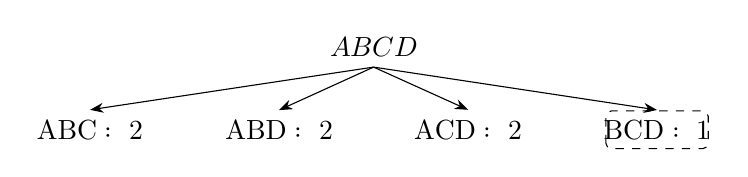
\begin{tikzpicture}[x=1cm,y=1cm,>=Stealth, every node/.style={font=\normalsize}]
\node (top) at (0,1.05) {$ABCD$};
\foreach \name/\x/\val in {ABC/-3.6/2,ABD/-1.2/2,ACD/1.2/2,BCD/3.6/1}{
  \node (\name) at (\x,0) {\(\mathrm{\name}:\ \val\)};
  \draw[->] (top.south) -- (\name.north);
}
\draw[dashed,rounded corners=2pt] (2.95,-.24) rectangle (4.25,.24);
\end{tikzpicture}
\end{diagram}
Ngưỡng $s=2$. Ba bộ ba đạt ngưỡng, riêng $BCD$ chỉ có trong giỏ $ABCD$. Một tập con trượt ngưỡng là đủ để bỏ $ABCD$ trước lần quét tiếp theo.
\end{example}

\ask{Pr1}{Pr1(a,c)}{}
\original{DSA5101 Exam Practice Questions.pdf}{2}{53 536.890 542 756.890}
\original{DSA5101 Exam Practice Questions.pdf}{2}{53 430.890 542 476.890}
\answer{\maptag{answer:Pr1}}
\begin{guidesteps}[beginpenalty=10000]
\item \guidepart{(a)}Đếm giỏ chứa toàn bộ bộ ba: $ABC$ có ở giỏ 1, 2 nên support 2; $BCD$ chỉ có ở giỏ 2 nên support 1.
\item So với $s=2$ và dùng hai support đã cho: $L_3=\{ABC,ABD,ACD\}$. Cắt $ABCD$ ngay vì tập con $BCD\notin L_3$.
\end{guidesteps}
\begin{guidesteps}
\item \guidepart{(c)}Nhân đôi dữ liệu: tử và mẫu trong confidence đều nhân 2, nên support count gấp đôi còn confidence giữ nguyên.
\item Xem mỗi giỏ là một tập: ba la bàn trong một giỏ vẫn chỉ đóng góp 1 vào support của $C$.
\end{guidesteps}

\ask{P25-Q1}{P25-Q1(a,b)}{}
\original{2526Sem1-DSA5101.pdf}{2}{53 543.890 542 749.890}
\original{2526Sem1-DSA5101.pdf}{2}{53 223.890 542 322.890}
\answer{\maptag{answer:P25-Q1}\maptag{answer:P25-Q1ab}}
\begin{guidesteps}[beginpenalty=10000]
\item \guidepart{(a)}Quét các giỏ để đếm singleton, giữ những item có support ít nhất 3. Dùng $L_1$ để sinh các cặp trong $C_2$ rồi đếm lại.
\item Chỉ giữ bộ ba có mọi cặp thuộc $L_2$: $ABD$. Đếm được 3 nên giữ. Không còn ứng viên cỡ 4.
\begin{examtable}{@{}c l l@{}}
\toprule
$k$ & $C_k$ và support tương ứng & $L_k$ \\
\midrule
1 & $A,B,C,D,E:\ 5,6,3,4,2$ & $A,B,C,D$ \\
2 & $AB,AC,AD,BC,BD,CD:\ 5,2,3,3,4,2$ & $AB,AD,BC,BD$ \\
3 & $ABD:\ 3$ & $ABD$ \\
4 & $\varnothing$ & $\varnothing$ \\
\bottomrule
\end{examtable}
\item Đọc kết quả từ các cột $L_k$: tập frequent là $L_1\cup L_2\cup L_3$.
\end{guidesteps}
\begin{guidesteps}
\item \guidepart{(b)}Tách hai việc: sinh và cắt ứng viên dùng kết quả trong bộ nhớ; đếm support mới cần quét giỏ trên đĩa.
\item Có ba mức cần đếm, nên quét 3 lượt. Vì $C_4$ rỗng, không quét thêm.
\end{guidesteps}

\ask{P25-Q1g}{P25-Q1(g)}{Dữ kiện chung: \hyperref[question:P25-Q1]{[P25-Q1]}}
\original{2526Sem1-DSA5101.pdf}{3}{53 284.890 542 425.890}
\answer{\maptag{answer:P25-Q1g}}
\begin{guidesteps}[beginpenalty=10000]
\item \guidepart{(g)}Tính khoảng giá $R(X)=\max_{i\in X}p_i-\min_{i\in X}p_i$ ngay khi sinh $X$.
\item Nếu $R(X)\ge T$, bỏ $X$ và các tập chứa nó vì thêm item không thể làm giảm khoảng giá. Giữ các ứng viên còn lại rồi đếm support.
\end{guidesteps}

\ask[A1-Q1]{P24-Q1}{P24-Q1 / A1-Q1}{}
\original{2425Sem1-DSA5101.pdf}{2}{53 425.890 542 749.890}
\answer{\maptag{answer:A1-Q1}\maptag{answer:P24-Q1}}
\begin{guidesteps}[beginpenalty=10000]
\item Với mỗi tập $X$, so support của các tập con đã biết với $s=5$. Nếu một tập con có support dưới 5, $X$ chắc chắn không frequent.
\item Nếu chỉ có cận trên bằng hoặc lớn hơn 5, chưa đủ kết luận. Áp dụng cho từng hàng:
\begin{examtable}{@{}l l l@{}}
\toprule
Tập & Điền vào cột & Lý do \\
\midrule
$ac$ & Không đủ thông tin & Tần suất riêng không cho biết giao. \\
$cd$ & Không đủ thông tin & Tần suất riêng không cho biết giao. \\
$bde$ & Không đủ thông tin & Support của $bd$ chỉ là cận trên. \\
$bcd$ & Chắc chắn không frequent & Chứa $bc$ có support $2<5$. \\
$abcd$ & Chắc chắn không frequent & Chứa $bc$ có support $2<5$. \\
\bottomrule
\end{examtable}
\item Không có hàng nào được bảo đảm frequent.
\end{guidesteps}

\topic{pairs}{Pair counters: triangular matrix vs triples}
\key{Khi dùng} So bộ nhớ để lưu số đếm của các cặp. Với $n$ item và $q$ cặp thực sự xuất hiện:
\begin{itemize}
\item Triangular matrix: có $\binom n2$ ô, mỗi ô 4 byte.
\item Triples: mỗi bản ghi $(i,j,\mathrm{count})$ tốn 12 byte; có $q$ bản ghi.
\end{itemize}
\key{So nhanh} Triples tiết kiệm khi $q<\binom n2/3$, chưa tính overhead. Với $n=4$, $q=2$ thì hòa (24 byte); $q=3$ thì bảng đặc rẻ hơn.



\topic{pcy}{PCY}
\key{Khi dùng} Tìm frequent pairs khi không đủ bộ nhớ giữ số đếm của mọi cặp.

\steps{
\item Pass 1: đếm item đơn và đưa mỗi cặp quan sát được vào bucket $h(i,j)$. Lưu bitmap: bit bằng 1 nếu số đếm bucket $\ge s$.
\item Pass 2: chỉ đếm chính xác cặp có cả hai item frequent và bit bucket bằng 1. So số đếm thật với $s$ để kết luận.
}
\key{Bẫy} Nhiều cặp có thể rơi vào cùng bucket. Bucket đủ ngưỡng chỉ cho phép giữ ứng viên; kết luận frequent cần số đếm của riêng cặp đó.

\ask{Pr2}{Pr2}{}
\original{DSA5101 Exam Practice Questions.pdf}{3}{53 550.890 542 784.890}
\answer{\maptag{answer:Pr2}}
\begin{guidesteps}[beginpenalty=10000]
\item \guidepart{(a)}So số đếm bucket $(1,2,3,4,2)$ với $s=3$: bitmap là $(0,0,1,1,0)$.
\item Chỉ xét cặp từ $\{1,2,4\}$. Các cặp $12,14,24$ băm vào bucket $2,4,3$; giữ $12,24$ và bỏ $14$, cặp mà Apriori vẫn đếm.
\end{guidesteps}
\begin{guidesteps}
\item \guidepart{(b)}Đếm giỏ chứa $12$ (giỏ 1, 2, 3) và $24$ (giỏ 3, 5): support là 3 và 2; chỉ $12$ đạt ngưỡng.
\item Một bucket cộng lượt của nhiều cặp khác nhau, nên bản thân bucket đạt ngưỡng chưa đủ để kết luận cặp nào frequent.
\end{guidesteps}
\begin{guidesteps}
\item \guidepart{(c)}Apriori cần $3\cdot4=12$ byte; PCY cần $2\cdot12+1=25$ byte.
\item So tổng bộ nhớ: trong cách lưu này, phần ghi ID và bitmap khiến PCY tốn hơn dù đếm ít cặp hơn.
\end{guidesteps}

\topic{multihash}{Multistage \& Multihash (PCY refinements)}
\key{Ý chính} Kiểm tra nhiều bitmap: cặp frequent phải qua tất cả vì số đếm bucket chứa nó luôn ít nhất bằng support của cặp.
\steps{
\item Multistage (3 pass): tạo bitmap $B_1$ như PCY. Quét lần hai, chỉ băm các cặp qua bộ lọc PCY vào hàm $h_2$ để tạo $B_2$. Quét lần ba để đếm cặp qua cả hai bitmap.
\item Multihash (2 pass): dựng cả hai bảng băm cùng lúc ở pass 1; pass 2 đếm cặp qua cả hai bitmap. Cùng ngân sách bộ nhớ, mỗi bảng thường nhỏ hơn và dễ va chạm hơn.
}
\key{Bẫy} Thêm bảng không luôn tiết kiệm bộ nhớ. Nếu gần như mọi bit đã là 1 thì bitmap ít giúp cắt ứng viên.



\topic{toivonen}{Toivonen}
\key{Khi dùng} Muốn dùng mẫu nhỏ nhưng vẫn kiểm tra được liệu có bỏ sót frequent itemset hay không.

\steps{
\item Lấy mẫu, giảm ngưỡng support cho mẫu, rồi tìm họ tập frequent $F$ trong mẫu.
\item Tìm negative border: các tập $X\notin F$ mà mọi tập con thực sự, khác rỗng của $X$ đều nằm trong $F$. Nếu xét đủ miền item, một singleton vắng khỏi $F$ cũng thuộc border.
\item Quét toàn bộ dữ liệu một lần để đếm $F$ và border. Nếu có tập ở border đạt ngưỡng toàn cục thì bỏ mẫu và chạy lại. Nếu không, trả các tập của $F$ đạt ngưỡng toàn cục.
}
\key{Vì sao đúng} Nếu bỏ sót tập frequent, chọn tập con nhỏ nhất của nó cũng bị bỏ sót. Tập này thuộc border và cũng frequent, nên lượt kiểm tra sẽ phát hiện.

\hard{P25-Q1cdf}{Tìm border theo từng kích thước}
Kiểm tra singleton trên toàn miền item trước. Ở mức $k>1$, ghép từ $F_{k-1}$, giữ ứng viên có mọi tập con kích thước $k-1$ thuộc $F_{k-1}$, rồi lấy hiệu với $F_k$. Tính đóng xuống của $F$ bảo đảm các tập con nhỏ hơn cũng nằm trong $F$. Trong P25-Q1(d), $E$ thuộc border vì không có tập con khác rỗng; $AC,CD$ cũng thuộc border; $ACD$ không thuộc vì $AC$ đã trượt. Khi chạy thành công, phải lọc lại cả $F$ bằng support toàn cục để loại sai dương.

\begin{example}{Pr3}{Pr3(a,b) · Toivonen: đọc negative border}
\begin{examtable}{@{}l l l@{}}
\toprule
Tập đang xét & Kiểm tra trên mẫu & Kết luận \\
\midrule
$AC$ & $A,C$ frequent; $AC$ không & Thuộc negative border \\
$ABC$ & $AC$ không frequent & Không thuộc border \\
\bottomrule
\end{examtable}
Quét đủ 10 tài liệu: $\operatorname{supp}(AC)=5$, đạt ngưỡng toàn cục. Bỏ lượt chạy và lấy mẫu lại; nếu không kiểm tra border, còn bỏ sót cả $ABC$ (support $5$).
\end{example}

\ask{Pr3}{Pr3}{}
\original{DSA5101 Exam Practice Questions.pdf}{4}{53 515.890 542 784.890}
\answer{\maptag{answer:Pr3}}
\begin{guidesteps}[beginpenalty=10000]
\item \guidepart{(a)}Các singleton đều thuộc $F$. Liệt kê cặp chưa có: $AC,BD,CD$; cả ba vào negative border.
\item Thử $ABC$: tập con $AC$ vắng trong $F$, nên $ABC$ không vào border. Mọi bộ ba khác cũng chứa một cặp vắng.
\end{guidesteps}
\begin{guidesteps}
\item \guidepart{(b)}Quét toàn bộ: $AC$ và $ABC$ cùng xuất hiện trong tài liệu 1, 6, 7, 8, 9; cả hai có support 5.
\item Vì $AC$ thuộc border và đạt ngưỡng 5, phải lấy mẫu lại. Bỏ qua phép thử sẽ bỏ sót bộ ba frequent $ABC$.
\end{guidesteps}
\begin{guidesteps}
\item \guidepart{(c)}Giả sử $S$ globally frequent nhưng vắng trong $F$. Chọn tập con $T\subseteq S$ nhỏ nhất vẫn vắng trong $F$.
\item Mọi tập con thực sự không rỗng của $T$ đều có trong $F$, nên $T$ thuộc border. Hơn nữa $\operatorname{supp}(T)\ge\operatorname{supp}(S)$, nên quét border sẽ phát hiện.
\end{guidesteps}

\ask{P25-Q1cdf}{P25-Q1(c-f)}{Dữ kiện chung: \hyperref[question:P25-Q1]{[P25-Q1]}}
\original{2526Sem1-DSA5101.pdf}{2}{53 126.890 542 145.890}
\original{2526Sem1-DSA5101.pdf}{3}{53 661.890 542 738.890}
\original{2526Sem1-DSA5101.pdf}{3}{53 554.890 542 603.890}
\original{2526Sem1-DSA5101.pdf}{3}{53 465.890 542 496.890}
\answer{\maptag{answer:P25-Q1cdf}}
\begin{guidesteps}[beginpenalty=10000]
\item \guidepart{(c)}Đào trên mẫu nhỏ để tìm họ frequent và border. Sau đó quét toàn dữ liệu một lượt để xác nhận, thay vì một lượt cho từng mức như Apriori.
\end{guidesteps}
\begin{guidesteps}
\item \guidepart{(d)}Kiểm tra singleton trước: $E$ không frequent nên thuộc border. Kiểm tra cặp: $AC,CD$ trượt nhưng cả hai singleton của từng cặp đều đạt.
\item Mỗi bộ ba trượt có một cặp trượt, nên không thuộc border. Kết quả $\{E,AC,CD\}$.
\end{guidesteps}
\begin{guidesteps}
\item \guidepart{(e)}Đếm support toàn cục của border. Nếu một tập đạt ngưỡng toàn cục, bỏ mẫu và lấy lại.
\item Giảm ngưỡng mẫu để giảm khả năng bỏ sót, đổi lại phải xác nhận nhiều ứng viên hơn.
\end{guidesteps}
\begin{guidesteps}
\item \guidepart{(f)}Giả sử vẫn bỏ sót tập globally frequent và chọn tập con nhỏ nhất bị bỏ sót. Tập con này thuộc border và cũng globally frequent.
\item Điều đó trái với việc xác nhận thành công, nên xác suất bỏ sót khi đã xác nhận là $0\%$.
\end{guidesteps}

\topic{son}{Random Sampling \& SON}
\key{Phân biệt}
\begin{itemize}
\item Random sampling: đào trên một mẫu chiếm tỷ lệ $p$, với ngưỡng khoảng $ps$. Quét xác nhận chỉ lọc sai dương trong các ứng viên đã tìm; một tập vắng khỏi mẫu vẫn có thể bị bỏ sót.
\item SON: chia toàn bộ dữ liệu thành các phần vừa bộ nhớ. Pass 1 lấy hợp các tập đạt ngưỡng $p_js$ ở phần $j$; $p_j$ là tỷ lệ giỏ ở phần đó. Pass 2 đếm toàn cục cho hợp ứng viên, giữ tập có support $\ge s$.
\end{itemize}
\key{Vì sao SON không bỏ sót} Nếu mọi support cục bộ đều $<p_js$, cộng lại sẽ $<s$. Ví dụ hai phần bằng nhau và $s=6$: ngưỡng mỗi phần là 3; một tập có tổng 6 phải đạt ít nhất 3 ở một phần.



\topic{rules}{Association rules}
\key{Khi dùng} Đề hỏi luật $X\to y$. Đặt $a=\operatorname{supp}(X)$, $c=\operatorname{supp}(X\cup\{y\})$, $p_y=\operatorname{supp}(y)/N$ với $N$ là số giỏ.
\[
\begin{aligned}
\operatorname{conf}(X\to y)&=c/a,\\
\operatorname{interest}(X\to y)&=c/a-p_y,\\
\operatorname{lift}(X\to y)&=(c/a)/p_y .
\end{aligned}
\]
\key{Bẫy} Support của luật là $c$, không phải $a$. Công thức interest ở trên là dạng có dấu; dùng đúng định nghĩa đề cho. Lift cần $p_y>0$.

\ask{Pr1b}{Pr1(b)}{Dữ kiện chung: \hyperref[question:Pr1]{[Pr1]}}
\original{DSA5101 Exam Practice Questions.pdf}{2}{53 476.890 542 536.890}
\answer{\maptag{answer:Pr1b}}
\begin{guidesteps}[beginpenalty=10000]
\item \guidepart{(b)}Lấy support của hợp chia support vế trái: $\operatorname{conf}(BD\to A)=2/2=1$, $\operatorname{conf}(AC\to D)=2/3$.
\item Trừ tần suất tương đối của vế phải: hai signed interest là $1-5/7=2/7$ và $2/3-4/7=2/21$.
\item Hai luật đều có support count 2, nhưng chỉ $BD\to A$ đạt confidence $4/5$.
\end{guidesteps}

\lecture{2}{Finding similar items / LSH}

\topic{jaccard}{Shingling \& Jaccard}
\key{Khi dùng} Đề yêu cầu so độ giống của hai tài liệu theo các cụm $k$ token liên tiếp ($k$-shingles).
\steps{
\item Xác định token là ký tự hay từ. Trượt cửa sổ dài $k$ và lấy tập các shingle khác nhau.
\item Đếm số shingle chung và kích thước hợp.
}
\[
J(A,B)=\frac{|S_A\cap S_B|}{|S_A|+|S_B|-|S_A\cap S_B|}.
\]
\key{Ví dụ} \literal{ABCAB} với $k=2$ cho $\{AB,BC,CA\}$. $AB$ lặp nhưng chỉ đếm một lần.

\ask{Pr4}{Pr4(a)}{}
\original{DSA5101 Exam Practice Questions.pdf}{5}{53 624.890 542 756.890}
\answer{\maptag{answer:Pr4}}
\begin{guidesteps}[beginpenalty=10000]
\item \guidepart{(a)}Trượt cửa sổ 3 ký tự trên $D_3$: $ATG,TGA,GAC,ACA$ ứng với ID $7,8,3,4$.
\item So $S_3=\{3,4,7,8\}$ với $S_1=\{1,2,3,4\}$. Giao là $\{3,4\}$ và hợp có 6 phần tử, nên $J=2/6=1/3$.
\end{guidesteps}

\ask[A1-Q2]{P24-Q2}{P24-Q2(a) / A1-Q2(a)}{}
\original{2425Sem1-DSA5101.pdf}{6}{53 597.890 542 747.890}
\answer{\maptag{answer:A1-Q2}\maptag{answer:A1-Q2a}\maptag{answer:P24-Q2}\maptag{answer:P24-Q2a}}
\begin{guidesteps}[beginpenalty=10000]
\item \guidepart{(a)}Trượt hai từ mỗi lần. $D_1$: \literal{expected this}, \literal{this exam}, \literal{exam to}, \literal{to be}, \literal{be very}, \literal{very difficult}.
\item Làm tương tự với $D_2$: \literal{this exam}, \literal{exam is}, \literal{is not}, \literal{not difficult}.
\item Chỉ \literal{this exam} thuộc giao. Hợp có $6+4-1=9$ phần tử, nên $J=1/9$.
\end{guidesteps}

\ask{P25-Q2}{P25-Q2(a)(i)}{}
\original{2526Sem1-DSA5101.pdf}{4}{53 643.890 542 750.890}
\answer{\maptag{answer:P25-Q2}\maptag{answer:P25-Q2a}}
\begin{guidesteps}[beginpenalty=10000]
\item \guidepart{(a)(i)}Lấy 200 shingle chung làm tử số. Tính hợp $400+800-200=1000$ để không đếm giao hai lần.
\item Chia giao cho hợp: $J=200/1000=0.2$.
\end{guidesteps}

\topic{minhash}{MinHash}
\key{Khi dùng} Đề cho ma trận hàng là shingle, cột là tài liệu, hoặc cho sẵn các tập ID và hoán vị.

\steps{
\item Duyệt các hàng theo thứ tự $\pi$, dùng cùng $\pi$ cho tất cả tài liệu.
\item Với mỗi tài liệu, ghi ID của hàng có mặt đầu tiên để tạo một hàng chữ ký. Lặp với $t$ hoán vị; ước lượng $\widehat J$ bằng số hàng trùng chia $t$.
}
\key{Vì sao được} Hàng đầu tiên trong hợp rơi vào giao với xác suất $J(A,B)$; đúng lúc đó MinHash trùng. Ví dụ thứ tự $(1,4,3,2)$ trên tập $\{2,4\}$ trả ID 4, không phải vị trí 2. Chữ ký của $n$ tài liệu lưu $O(tn)$ giá trị.

\ask{Pr4bc}{Pr4(b,c)}{Dữ kiện chung: \hyperref[question:Pr4]{[Pr4]}}
\original{DSA5101 Exam Practice Questions.pdf}{5}{53 511.890 542 624.890}
\answer{\maptag{answer:Pr4bc}}
\begin{guidesteps}[beginpenalty=10000]
\item \guidepart{(b)}Duyệt theo mỗi hoán vị, ghi hàng đầu tiên có mặt trong từng tập. Với $\pi_1$, $5$ chỉ có trong $S_2$, còn $3$ gặp trước trong $S_1,S_3$: hàng chữ ký $(3,5,3)$.
\item Với $\pi_2$, $2$ gặp trước trong $S_1,S_2$, còn $7$ gặp trước trong $S_3$: hàng $(2,2,7)$. Cột 1 và 3 trùng 1 trong 2 hàng, nên ước lượng là $1/2$.
\end{guidesteps}
\begin{guidesteps}
\item \guidepart{(c)}Dùng cùng hoán vị để hai tập nhìn thấy cùng phần tử đến trước trong hợp. Hai chữ ký bằng nhau đúng khi phần tử đó thuộc giao.
\item Xác suất bằng nhau là $J=1/3$; hai lần thử vẫn có thể cho tần suất quan sát $1/2$.
\end{guidesteps}

\begin{example}{A1-Q2b}{A1-Q2(b) · MinHash: lấy ID hàng đầu tiên}
Với thứ tự thăm $3,5,1,4,2,6$, hàng có số 1 đầu tiên của $D_1$ là 5, dù nó đứng thứ hai trong thứ tự thăm.
\begin{examtable}{@{}l c c c c@{}}
\toprule
Cột & $D_1$ & $D_2$ & $D_3$ & $D_4$ \\
\midrule
Các hàng có số 1 & $\{1,2,5\}$ & $\{2,4\}$ & $\{3,6\}$ & $\{4\}$ \\
Thứ tự thăm đến khi gặp 1 & $3,\mathbf5$ & $3,5,1,\mathbf4$ & $\mathbf3$ & $3,5,1,\mathbf4$ \\
Hàng chữ ký & 5 & 4 & 3 & 4 \\
\bottomrule
\end{examtable}
\end{example}

\ask[A1-Q2b]{P24-Q2b}{P24-Q2(b) / A1-Q2(b)}{}
\original{2425Sem1-DSA5101.pdf}{6}{53 288.890 542 450.890}
\original{2425Sem1-DSA5101.pdf}{6}{53 64.890 542 278.890}
\answer{\maptag{answer:A1-Q2b}\maptag{answer:P24-Q2b}}
\begin{guidesteps}[beginpenalty=10000]
\item \guidepart{(b)}Đọc mỗi cột của $\pi$ như thứ tự thăm hàng. Với cột đầu, duyệt $3,5,1,4,2,6$.
\item Trong mỗi tài liệu, dừng tại hàng đầu có 1 và ghi ID hàng. Với $D_1$, hàng 5 được thăm thứ hai nhưng chữ ký là 5. Với $D_2,D_3,D_4$, ghi $4,3,4$.
\item Lặp lại với hai cột còn lại để được:
\[
M=\begin{pmatrix}5&4&3&4\\2&2&3&4\\1&4&3&4\end{pmatrix}.
\]
\end{guidesteps}

\topic{banding}{LSH banding}
\key{Khi dùng} Cần chọn cặp ứng viên từ chữ ký MinHash, tránh so chính xác mọi cặp.
\steps{
\item Chia $m=br$ số hash thành $b$ band, mỗi band $r$ hàng.
\item Một band khớp khi tất cả $r$ hàng khớp. Một cặp là ứng viên khi ít nhất một band khớp. So chính xác chỉ để xác nhận các ứng viên.
}
\[
\Pr(\mathrm{candidate}\mid s)=1-(1-s^r)^b.
\]
\key{Đọc tham số} $s$ là Jaccard, công thức giả sử các hàng độc lập. Tại $m$ cố định, tăng $b$ làm giảm $r$: thường tăng recall và giảm precision. Nếu $r$ cố định, tăng $b$ cũng tăng xác suất thành ứng viên.

\key{Mốc 50\%} $s_{1/2}=(1-2^{-1/b})^{1/r}$. Đây là mốc xác suất, không phải ngưỡng cứng. Bước xác nhận lọc ứng viên sai, không phục hồi cặp chưa từng được chọn.

\hard{P24-Q2cd}{Chọn cấu hình theo hai vùng similarity}
Nếu có ngân sách $m$ hash cố định, liệt kê các cặp nguyên $br=m$, rồi tính $P_{b,r}(s)$ ở similarity thấp và cao. Với $m=32$ trong P24-Q2/A1-Q2, $(b,r)=(8,4)$ cho $(P(0.2),P(0.6))\approx(0.01273,0.6706)$; đổi sang $(4,8)$ cho $(0.00001024,0.06551)$. Ít cặp không giống lọt qua hơn, nhưng nhiều cặp giống cũng bị mất. $P(s)$ là xác suất thành ứng viên tại $s$, không phải precision của cả tập kết quả.

\begin{example}{Pr5}{Pr5(a,b) · Banding: ứng viên và kết quả xác nhận}
\begin{examtable}{@{}l c c c l@{}}
\toprule
Cặp & Band 1 & Band 2 & Band 3 & So Jaccard với $3/5$ \\
\midrule
$AB$ & Có & -- & Có & $3/5$: giữ \\
$BD$ & -- & Có & -- & $2/5$: loại \\
$AC$ & -- & -- & -- & $3/5$: bị bỏ sót \\
\bottomrule
\end{examtable}
Gộp và bỏ trùng sau khi băm: chỉ so chính xác $AB$ và $BD$ (2 trên 6 cặp). $J(A,C)=3/5$ là kết quả kiểm tra lại; LSH không gửi cặp này sang bước xác nhận.
\end{example}

\ask{Pr5}{Pr5}{}
\original{DSA5101 Exam Practice Questions.pdf}{6}{53 472.890 542 784.890}
\answer{\maptag{answer:Pr5}}
\begin{guidesteps}[beginpenalty=10000]
\item \guidepart{(a)}Ghép hàng $(1,2),(3,4),(5,6)$ thành ba band. So từng tuple: các cặp trùng theo thứ tự là $AB,BD,AB$.
\item Gộp và bỏ trùng, còn $\{AB,BD\}$: cần 2 lần so chính xác thay vì 6.
\end{guidesteps}
\begin{guidesteps}
\item \guidepart{(b)}Đếm giao và hợp: $J(A,B)=3/5$ đạt ngưỡng; $J(B,D)=2/5$ bị loại. $BD$ là ứng viên dương giả.
\item $J(A,C)=3/5$ nhưng $AC$ không vào tập ứng viên, nên là âm giả. Bước xác nhận không khôi phục cặp đã bỏ sót.
\end{guidesteps}
\begin{guidesteps}
\item \guidepart{(c)}Một band khớp với xác suất $(1/2)^2=1/4$. Lấy bù của sự kiện cả ba band đều trượt: $1-(3/4)^3=37/64$.
\item Xác suất này nằm giữa 0 và 1; ngưỡng Jaccard không phải ranh giới tất định cho bước sinh ứng viên.
\end{guidesteps}

\ask[A1-Q2cd]{P24-Q2cd}{P24-Q2(c,d) / A1-Q2(c,d)}{}
\original{2425Sem1-DSA5101.pdf}{7}{53 515.890 542 596.890}
\original{2425Sem1-DSA5101.pdf}{7}{53 397.890 542 443.890}
\original{2425Sem1-DSA5101.pdf}{7}{53 111.890 542 312.890}
\answer{\maptag{answer:A1-Q2cd}\maptag{answer:P24-Q2cd}}
\begin{guidesteps}[beginpenalty=10000]
\item \guidepart{(c)(i)}Một band cần bốn hàng cùng khớp nên xác suất là $0.6^4$. Lấy bù của tám band đều trượt: $1-(1-0.6^4)^8\approx0.6706$.
\end{guidesteps}
\begin{guidesteps}
\item \guidepart{(c)(ii)}Thay $s=0.2$ vào cùng hai bước: band khớp với xác suất $0.2^4$; ít nhất một band khớp với xác suất $1-(1-0.2^4)^8\approx0.01273$.
\end{guidesteps}
\begin{guidesteps}
\item \guidepart{(d)}Giữ $m=br$ không đổi. Giảm $b$ làm $r$ tăng và còn ít band hơn để thử.
\item Chọn B: giảm $b$ để bớt ứng viên dương giả; đổi lại có thể bỏ sót nhiều cặp thật hơn.
\end{guidesteps}

\ask{P25-Q2aii}{P25-Q2(a)(ii,iii)}{Dữ kiện chung: \hyperref[question:P25-Q2]{[P25-Q2]}}
\original{2526Sem1-DSA5101.pdf}{4}{53 527.890 542 574.890}
\original{2526Sem1-DSA5101.pdf}{4}{53 424.890 542 471.890}
\answer{\maptag{answer:P25-Q2aii}}
\begin{guidesteps}[beginpenalty=10000]
\item \guidepart{(a)(ii)}Một band 10 hàng khớp với xác suất $0.2^{10}$. Lấy bù của 12 band độc lập đều trượt: $1-(1-0.2^{10})^{12}\approx1.229\times10^{-6}$.
\end{guidesteps}
\begin{guidesteps}
\item \guidepart{(a)(iii)}Tăng $b$ để có thêm cơ hội khớp. Nếu tổng số hash cố định, $r$ giảm nên mỗi band cũng dễ khớp hơn.
\end{guidesteps}

\topic{families}{LSH families, AND/OR amplification \& cascades}
\key{Khi dùng} Đề cho xác suất va chạm $p$ của một hash rồi ghép nhiều hash độc lập. Một họ LSH $(d_1,d_2,p_1,p_2)$ bảo đảm xác suất trùng $\ge p_1$ khi khoảng cách $\le d_1$ và $\le p_2$ khi khoảng cách $\ge d_2$.

\begin{itemize}
\item AND $r$ lần: tất cả trùng, xác suất $p^r$.
\item OR $b$ lần: ít nhất một lần trùng, xác suất $1-(1-p)^b$.
\item Cascade: áp dụng theo thứ tự từ tầng trong ra ngoài. Số hash gốc bằng tích số nhánh các tầng, nếu mỗi nhánh dùng hash độc lập.
\end{itemize}
\key{Ví dụ} Với $p=1/2$, dùng 2 nhánh mỗi tầng: AND rồi OR cho $7/16$; OR rồi AND cho $9/16$. Điểm bất động $f(s)=s$ khác mốc $f(s)=1/2$.

\hard{P24-Q2ef}{Tính cascade từ trong ra ngoài}
Mỗi tầng nhận xác suất đầu ra của tầng trước; đặt $p_1=0.9^5=0.59049$, $p_2=1-(1-p_1)^6\approx0.9953$ rồi $p_3=p_2^7\approx0.9675$. Mỗi nút OR chứa 6 nhánh AND độc lập, và có 7 bản sao của nút OR, nên cần $5\cdot6\cdot7=210$ hash gốc. Gắn thêm OR 3 rồi AND 4 nhân tiếp $12$, ra $2520$. Nếu dùng lại một hash, không được nhân xác suất như với các biến độc lập.

\ask[A1-Q2ef]{P24-Q2ef}{P24-Q2(e,f) / A1-Q2(e,f)}{}
\original{2425Sem1-DSA5101.pdf}{8}{53 636.890 542 741.890}
\original{2425Sem1-DSA5101.pdf}{8}{53 326.890 542 397.890}
\answer{\maptag{answer:P24-Q2ef}\maptag{answer:A1-Q2ef}}
\begin{guidesteps}[beginpenalty=10000]
\item \guidepart{(e)}Tính từ tầng trong ra: AND 5 cho $p_1=0.9^5$; OR 6 cho $p_2=1-(1-p_1)^6$.
\item AND 7 yêu cầu cả bảy nhánh cùng qua, nên xác suất là $p_2^7\approx0.9675$.
\end{guidesteps}
\begin{guidesteps}
\item \guidepart{(f)}Đếm lá thay vì cộng số tầng. Mỗi tầng nhân tiếp số nhánh, kể cả hai tầng mới 3 và 4: cần $5\cdot6\cdot7\cdot3\cdot4=2520$ hash gốc.
\end{guidesteps}

\topic{hyperplanes}{Random hyperplanes (cosine LSH)}
\key{Khi dùng} So vectơ theo góc; mỗi pháp tuyến $v$ cho một bit $h_v(x)=\operatorname{sign}(v^Tx)$.

\key{Cách làm} Nếu đề cho $v$, tính tích vô hướng rồi lấy dấu theo quy ước của đề. Nếu hỏi xác suất trên siêu phẳng ngẫu nhiên qua gốc, tính $\theta$ từ cosine:
\[
\cos\theta=\frac{x^Ty}{\|x\|\|y\|},\qquad
\Pr[h_v(x)=h_v(y)]=1-\theta/\pi.
\]
\key{Bẫy} Hai vectơ vuông góc trùng bit với xác suất $1/2$. Nhân vectơ với số dương giữ nguyên dấu. Lặp lại cùng siêu phẳng không tạo các phép thử độc lập.

\begin{example}{P25-Q2b}{P25-Q2(b) · Random hyperplanes: góc quyết định xác suất}
\begin{diagram}
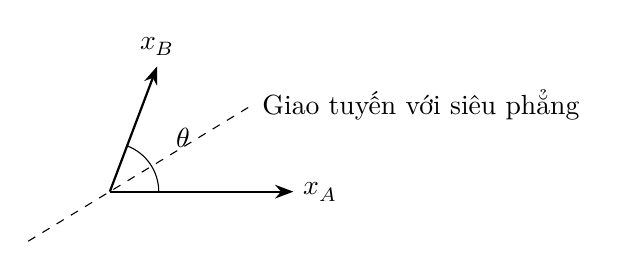
\begin{tikzpicture}[scale=.74,>=Stealth,every node/.style={font=\normalsize}]
\draw[dashed] (-1.4,-.85) -- (2.45,1.49) node[right] {Giao tuyến với siêu phẳng};
\draw[->,thick] (0,0) -- (3.15,0) node[right] {$x_A$};
\draw[->,thick] (0,0) -- (69.3:2.3) node[above] {$x_B$};
\draw (0.84,0) arc[start angle=0,end angle=69.3,radius=.84];
\node at (1.26,.93) {$\theta$};
\end{tikzpicture}
\end{diagram}
Hai vectơ có 200 vị trí cùng bằng 1, nên $\cos\theta=200/\sqrt{400\cdot800}=1/\sqrt8$ và $\theta\approx69.3^\circ$. Trong mặt phẳng chứa hai vectơ, giao tuyến đi qua gốc và tách chúng khi hướng của nó nằm trong góc $\theta$ (hướng xét theo modulo $180^\circ$). Vì vậy xác suất cùng phía là $1-\theta/180^\circ\approx0.615$.
\end{example}

\ask{Pr6}{Pr6}{}
\original{DSA5101 Exam Practice Questions.pdf}{7}{53 589.890 542 784.890}
\answer{\maptag{answer:Pr6}}
\begin{guidesteps}[beginpenalty=10000]
\item \guidepart{(a)}Tính $v_i\cdot Q$ cho bốn pháp tuyến: $(2,2,-2,6)$. Lấy dấu được $(+,+,-,+)$.
\item So với chữ ký của $P$: trùng ở vị trí 1, 2, 4 nên tỉ lệ là $3/4$.
\end{guidesteps}
\begin{guidesteps}
\item \guidepart{(b)}AND rồi OR: xác suất mỗi cặp qua AND là $p^2=1/4$; ít nhất một cặp qua với xác suất $1-(3/4)^2=7/16$.
\item OR rồi AND: mỗi cặp qua OR với xác suất $1-(1-p)^2=3/4$; cả hai qua với xác suất $(3/4)^2=9/16$.
\end{guidesteps}
\begin{guidesteps}
\item \guidepart{(c)}Dùng lại cùng mặt phẳng làm các bit phụ thuộc, nên không nhân xác suất như với bốn mặt phẳng độc lập.
\item Thay $Q$ bằng $10Q$ nhân mọi tích vô hướng với 10, không đổi dấu hay chữ ký.
\end{guidesteps}

\ask{P25-Q2b}{P25-Q2(b)}{Dữ kiện chung: \hyperref[question:P25-Q2]{[P25-Q2]}}
\original{2526Sem1-DSA5101.pdf}{4}{53 326.890 542 400.890}
\answer{\maptag{answer:P25-Q2b}}
\begin{guidesteps}[beginpenalty=10000]
\item \guidepart{(b)}Dùng vectơ hiện diện: tích vô hướng là 200, bình phương chuẩn là 400 và 800. Suy ra $\cos\theta=200/\sqrt{400\cdot800}=1/\sqrt8$.
\item Đổi góc sang xác suất hai vectơ cùng phía: $1-\arccos(1/\sqrt8)/\pi\approx0.6150$.
\end{guidesteps}

\topic{euclidean}{Euclidean-distance LSH via random projection}
\key{Khi dùng} Tìm cặp vectơ gần nhau theo khoảng cách Euclid bằng phép chiếu lên đường thẳng.

\key{Cách làm} Chiếu $x$ lên hướng $u$, chia đường chiếu thành các ô rộng $a$ và băm vào số ô. Ví dụ nếu mốc ô là 0 thì $h_u(x)=\lfloor u^Tx/a\rfloor$. Với $a=2$, các giá trị chiếu $1.3,1.8,2.1$ vào các ô $0,0,1$.

\key{Bẫy} Hai điểm gần nhau vẫn có thể nằm hai bên biên ô. Trong mô hình của lecture, các mốc gần/xa $a/2$ và $2a$ cho cận va chạm lần lượt $\ge1/2$ và $\le1/3$.



\lecture{3}{Clustering}

\topic{hierarchical}{Hierarchical agglomerative clustering}
\key{Khi dùng} Đề yêu cầu cây gộp cụm (dendrogram). Bắt đầu từ các cụm một điểm; mỗi vòng gộp hai cụm có khoảng cách linkage nhỏ nhất. Ghi khoảng cách đó làm độ cao của lần gộp.

\begin{itemize}
\item Single: lấy khoảng cách nhỏ nhất trong các cặp chéo hai cụm.
\item Complete: lấy khoảng cách lớn nhất trong các cặp chéo.
\item Average: lấy trung bình của mọi khoảng cách chéo.
\item Clustroid: chọn một điểm thật trong cụm, thường là điểm có tổng khoảng cách đến các điểm cùng cụm nhỏ nhất. So các điểm đại diện nếu đề yêu cầu clustroid linkage.
\end{itemize}
\key{Bẫy} Độ cao gộp theo single có thể nhỏ hơn đường kính của cụm vừa gộp. Khi hòa, theo đúng quy tắc của đề.

\hard{A1-Q3}{Cập nhật khoảng cách sau khi gộp}
Nếu $U=A\cup B$, single và complete lấy min và max của hai khoảng cách cũ tới $C$. Với average linkage theo mọi cặp điểm, dùng
\[
d(U,C)=\frac{|A|d(A,C)+|B|d(B,C)}{|A|+|B|}.
\]
Trong A1-Q3 với khoảng cách Euclid, từ $\{1,2,4\}$ tới $8$: single $=8-4=4$, complete $=8-1=7$, average $=(7+6+4)/3=17/3$. Khi đề đổi sang khoảng cách tỉ số, phải tính lại từ định nghĩa; dấu bằng giữa các khoảng cách kích hoạt quy tắc phá hòa của đề.

\begin{example}{A1-Q3}{A1-Q3(b) · Dendrogram: complete linkage với khoảng cách tỉ số}
\begin{diagram}
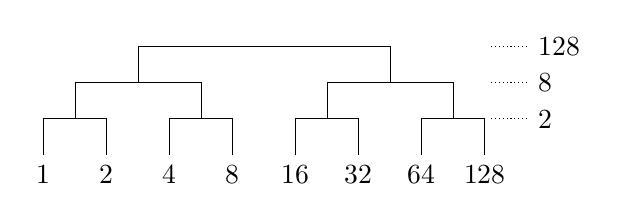
\begin{tikzpicture}[x=.80cm,y=.46cm, every node/.style={font=\normalsize}]
\foreach \i/\v in {0/1,1/2,2/4,3/8,4/16,5/32,6/64,7/128}
  \node[below] at (\i,0) {$\v$};
\foreach \i in {0,2,4,6}
  \draw (\i,0) -- (\i,1) -| ++(1,-1);
\foreach \i in {.5,4.5}
  \draw (\i,1) -- (\i,2) -| ++(2,-1);
\draw (1.5,2) -- (1.5,3) -| (5.5,2);
\foreach \y/\v in {1/2,2/8,3/128}{
  \draw[densely dotted] (7.1,\y) -- (7.7,\y) node[right] {$\v$};
}
\end{tikzpicture}
\end{diagram}
Chiều cao ghi theo $d(x,y)=\max(x,y)/\min(x,y)$, cách đều để dễ đọc. Khi gộp $\{1,2\}$ với $\{4,8\}$, cặp xa nhất là $(1,8)$ nên chiều cao là $8$.
\end{example}

\ask{Pr7}{Pr7}{}
\original{DSA5101 Exam Practice Questions.pdf}{8}{53 459.890 542 756.890}
\answer{\maptag{answer:Pr7}}
\begin{guidesteps}[beginpenalty=10000]
\item \guidepart{(a)}Single lấy $\min(5,3)=3$ cho khoảng cách $AB$ đến $C$. Vì $3<d(D,E)=4$ và các cặp còn lại lớn hơn 3, gộp $AB$ với $C$.
\item Clustroid của $AB$ là $A$ nên khoảng cách đến $C$ là 5. Cặp gần nhất lúc này là $D,E$ ở 4.
\end{guidesteps}
\begin{guidesteps}
\item \guidepart{(b)}Cộng khoảng cách đến các thành viên trong $ABC$: $A:7,B:5,C:8$. Chọn $B$ có tổng nhỏ nhất.
\item Lấy khoảng cách cặp lớn nhất, $d(A,C)=5$. Diameter có thể lớn hơn độ cao single linkage 3 khi $C$ nhập cụm.
\end{guidesteps}
\begin{guidesteps}
\item \guidepart{(c)}Tính tổng khoảng cách chỉnh sửa cho từng chuỗi có thật rồi chọn chuỗi nhỏ nhất theo tổng. Không cần định nghĩa trung bình của các chuỗi.
\end{guidesteps}

\ask[A1-Q3]{P24-Q3}{P24-Q3 / A1-Q3}{}
\original{2425Sem1-DSA5101.pdf}{12}{53 642.890 542 747.890}
\original{2425Sem1-DSA5101.pdf}{13}{53 718.890 542 748.890}
\original{2425Sem1-DSA5101.pdf}{13}{53 413.890 542 434.890}
\original{2425Sem1-DSA5101.pdf}{14}{53 576.890 542 738.890}
\answer{\maptag{answer:A1-Q3}\maptag{answer:P24-Q3}}
\begin{guidesteps}[beginpenalty=10000]
\item \guidepart{(a)(i)--(iii)}Bắt đầu với cặp gần nhất $1,2$. Khi đã gộp đến $2^{j-1}$, khoảng cách complete tới $2^j$ bằng $2^j-1$, nhỏ hơn khoảng cách $2^j$ của cặp singleton gần nhất còn lại. Single và average không lớn hơn complete, nên cả ba cùng ghép lần lượt $4,8,16,32,64,128$.
\item Tại nút $j$, lấy min, max hoặc trung bình khoảng cách chéo: $2^j-2^{j-1}$, $2^j-1$ hoặc $2^j-(2^j-1)/j$. Dùng bảng để đặt độ cao trên cây:
\begin{diagram}
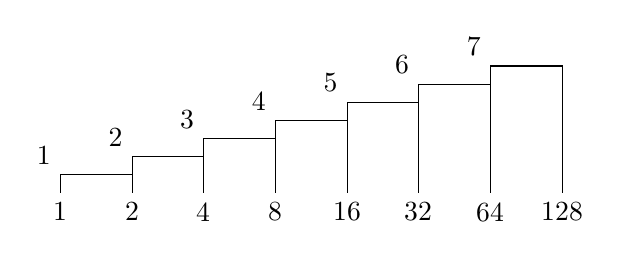
\begin{tikzpicture}[x=.91cm,y=.23cm,every node/.style={font=\normalsize}]
\node[below] at (0,0) {$1$};
\foreach \j/\v in {1/2,2/4,3/8,4/16,5/32,6/64,7/128}{
  \node[below] at (\j,0) {$\v$};
  \pgfmathtruncatemacro{\prev}{\j-1}
  \draw (\prev,\prev) -- (\prev,\j) -| (\j,0);
  \node[above left] at (\prev,\j) {\j};
}
\end{tikzpicture}
\end{diagram}
\begin{examtable}{@{}l c c c c c c c@{}}
\toprule
Nút $j$ & 1 & 2 & 3 & 4 & 5 & 6 & 7 \\
\midrule
(i) Single & 1 & 2 & 4 & 8 & 16 & 32 & 64 \\
(ii) Complete & 1 & 3 & 7 & 15 & 31 & 63 & 127 \\
(iii) Average & 1 & $5/2$ & $17/3$ & $49/4$ & $129/5$ & $321/6$ & $769/7$ \\
\bottomrule
\end{examtable}
\end{guidesteps}
\begin{guidesteps}
\item \guidepart{(b)}Đổi sang khoảng cách tỉ số và dùng complete: khoảng cách hai cụm là điểm lớn nhất chia điểm nhỏ nhất của cặp xa nhất.
\item Ở độ cao 2, phá hòa theo rank để gộp lần lượt $(1,2),(4,8),(16,32),(64,128)$. Gộp hai cặp đầu và hai cặp cuối ở 8, rồi hai cụm còn lại ở 128. Đối chiếu cây ở ví dụ ngay trước đề.
\end{guidesteps}

\topic{kmeans}{K-means / Lloyd's algorithm}
\key{Khi dùng} Đề cho $K$ tâm hoặc một cách gán điểm ban đầu. Mục tiêu là giảm SSE, tức tổng bình phương khoảng cách của mỗi điểm tới tâm cụm của nó.
\steps{
\item Assign: gán mỗi điểm vào tâm gần nhất.
\item Update: thay tâm của mỗi cụm $C$ bằng trung bình $\mu_C=\sum_{x\in C}x/|C|$.
\item Lặp cho đến khi không đổi hoặc mức giảm SSE đủ nhỏ. Xử lý cụm rỗng theo quy ước đề.
}
\key{Bẫy} Mỗi bước không tăng SSE, nhưng nghiệm dừng có thể không tối ưu toàn cục. Một vòng thường tốn $O(nKd)$ với $n$ điểm, $d$ chiều.

\hard{Pr8}{Phân biệt nghiệm dừng với tối ưu toàn cục}
So SSE trên cùng dữ liệu, lấy lại tâm cho mỗi phân hoạch. Trong Pr8(c), cụm $ABDE$ có bốn điểm ở khoảng cách bình phương 10 tới tâm $(3,1)$; cụm $CF$ có hai điểm ở khoảng cách bình phương 9 tới $(3,4)$. Tổng là $4\cdot10+2\cdot9=58$. Tách theo hai cột, mỗi tâm ở $y=2$; mỗi cột có SSE $4+0+4=8$. Một phân hoạch có SSE $16<58$ đủ bác bỏ tối ưu toàn cục, không cần chứng minh $16$ là nhỏ nhất.

\begin{example}{Pr8}{Pr8(a,b) · K-means: cập nhật tâm rồi gán lại $B$}
\begin{diagram}
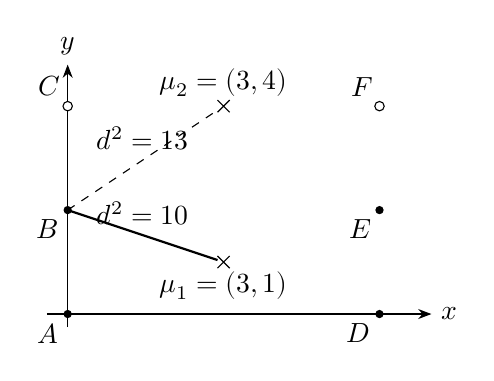
\begin{tikzpicture}[x=.66cm,y=.66cm,>=Stealth,every node/.style={font=\normalsize}]
\draw[->] (-.4,0) -- (7,0) node[right] {$x$};
\draw[->] (0,-.25) -- (0,4.8) node[above] {$y$};
\foreach \x/\y/\name in {0/0/A,0/2/B,6/0/D,6/2/E}
  \fill (\x,\y) circle (1.5pt) node[below left] {$\name$};
\foreach \x/\name in {0/C,6/F}
  \draw[fill=white] (\x,4) circle (1.7pt) node[above left] {$\name$};
\node[cross out,draw,inner sep=2pt] (mu) at (3,1) {};
\node[cross out,draw,inner sep=2pt] (nu) at (3,4) {};
\node[below] at (3,1) {$\mu_1=(3,1)$};
\node[above] at (3,4) {$\mu_2=(3,4)$};
\draw[thick] (0,2) -- (mu) node[midway,above] {$d^2=10$};
\draw[dashed] (0,2) -- (nu) node[midway,above] {$d^2=13$};
\end{tikzpicture}
\end{diagram}
Chấm đen: cụm $ABDE$; vòng rỗng: cụm $CF$; dấu chéo: tâm mới. Tâm mỗi cụm là trung bình tọa độ; $B$ ở lại cụm 1 vì $3^2+1^2<3^2+2^2$.
\end{example}

\ask{Pr8}{Pr8}{}
\original{DSA5101 Exam Practice Questions.pdf}{9}{53 626.890 542 787.890}
\answer{\maptag{answer:Pr8}}
\begin{guidesteps}[beginpenalty=10000]
\item \guidepart{(a)}Lấy trung bình tọa độ của $A,B,D,E$: tâm thứ nhất là $(3,1)$. Lấy trung bình của $C,F$: tâm thứ hai là $(3,4)$.
\end{guidesteps}
\begin{guidesteps}
\item \guidepart{(b)}Với $B=(0,2)$, tính bình phương khoảng cách tới hai tâm: $9+1=10$ và $9+4=13$. Giữ $B$ ở cụm 1.
\item Các điểm khác giữ cụm theo giả thiết. Thành viên không đổi nên lần cập nhật kế tiếp giữ nguyên hai tâm: đây là điểm dừng.
\end{guidesteps}
\begin{guidesteps}
\item \guidepart{(c)}So SSE của hai phân hoạch: $16<58$, nên điểm dừng không tối ưu toàn cục.
\item Thử nhiều khởi tạo rồi giữ nghiệm có SSE nhỏ nhất, hoặc dùng khởi tạo k-means++.
\end{guidesteps}

\topic{seeding}{K-means++-style seeding, choosing K \& stopping}
\key{Ý chính} Tâm ban đầu khác nhau có thể cho các nghiệm khác nhau. Chọn tâm đầu ngẫu nhiên; chọn điểm tiếp theo với xác suất tỷ lệ $D(x)^2$, trong đó $D(x)$ đo tới tâm đã chọn gần nhất.

\key{Tính nhanh} Nếu $D=(1,2,3)$, trọng số là $(1,4,9)$; chuẩn hóa bằng tổng 14. Điểm xa nhất có xác suất cao hơn chứ không được chọn chắc chắn.

\key{Quy ước} K-means++ chuẩn chọn $K$ tâm. Biến thể trong lecture lấy khoảng $K\log N$ điểm rồi gom mẫu để khởi tạo tâm. Khi chọn $K$, elbow là nơi tăng thêm cụm chỉ giảm SSE ít; có thể không có elbow rõ.



\topic{bfr}{BFR (Bradley-Fayyad-Reina)}
\key{Khi dùng} Dữ liệu lớn đọc theo lô; giữ thống kê của cụm thay cho từng điểm. BFR phù hợp cụm gần Gaussian theo các trục tọa độ.
\begin{itemize}
\item DS: các điểm đã gán vào cụm chính; chỉ giữ tóm tắt.
\item CS: các cụm tạm chưa gán vào cụm chính; cũng giữ tóm tắt.
\item RS: còn giữ từng điểm chưa gán để thử gom ở lô sau.
\end{itemize}
\key{Tính} Cộng các bộ $(N,\mathrm{SUM},\mathrm{SUMSQ})$ theo tọa độ để gộp. Sau đó tính
\[
\mu_j=\mathrm{SUM}_j/N,\quad \sigma_j^2=\mathrm{SUMSQ}_j/N-\mu_j^2,\quad
D_M^2=\sum_j\frac{(x_j-\mu_j)^2}{\sigma_j^2}.
\]
\key{Bẫy} So $D_M^2$ với ngưỡng bình phương nếu đề cho như vậy. Không chia trực tiếp cho phương sai bằng 0.

\hard{Pr9}{Gộp cụm có thể làm phương sai tăng}
Ở mỗi chiều, đặt $w_i=N_i/(N_1+N_2)$. Phương sai sau gộp là
\[
\sigma_{\rm gộp}^2=w_1\sigma_1^2+w_2\sigma_2^2+w_1w_2(\mu_1-\mu_2)^2.
\]
Hai cụm riêng lẻ có thể rất chặt nhưng tâm cách xa. Với hai CS trong Pr9(c), chiều thứ hai có trọng số bằng nhau, tâm $6.5,8.5$ và mỗi phương sai là $1/4$. Sau gộp được $1/4+(1/4)\cdot2^2=5/4>1$, nên không gộp. Tính được từ tóm tắt mà không cần điểm gốc.

\ask{Pr9}{Pr9}{}
\original{DSA5101 Exam Practice Questions.pdf}{10}{53 584.890 542 784.890}
\answer{\maptag{answer:Pr9}}
\begin{guidesteps}[beginpenalty=10000]
\item \guidepart{(a)}Chia SUM cho 4 để có $\mu=(0,0)$; lấy $\mathrm{SUMSQ}/4-\mu^2$ theo tọa độ để có phương sai $(1,4)$.
\item Tính $D_M^2(P)=1^2/1+2^2/4=2$. Giá trị này $\le4$ và nhỏ hơn $85/9$, nên đưa $P$ vào DS đã cho.
\end{guidesteps}
\begin{guidesteps}
\item \guidepart{(b)}Gộp cặp duy nhất đạt ngưỡng khoảng cách là $R,S$. Cộng tọa độ và bình phương tọa độ: CS có $(N,\mathrm{SUM},\mathrm{SUMSQ})=(2,(0,13),(0,85))$.
\item Giữ riêng $T=(15,8)$ trong RS.
\end{guidesteps}
\begin{guidesteps}
\item \guidepart{(c)}Cộng hai bộ thống kê: $N=4$, tổng tọa độ 2 là 30 và tổng bình phương là 230.
\item Tính $230/4-(30/4)^2=5/4>1$, nên không gộp. Các thống kê đã đủ để tính phương sai.
\end{guidesteps}

\ask{P25-Q7}{P25-Q7(a)}{}\maptag{question:P25-Q7a}
\original{2526Sem1-DSA5101.pdf}{18}{53 653.890 542 750.890}
\answer{\maptag{answer:P25-Q7}\maptag{answer:P25-Q7a}}
\begin{guidesteps}[beginpenalty=10000]
\item \guidepart{(a)}Xác định BFR dùng thống kê tóm tắt theo cụm và mở rộng k-means để xử lý dữ liệu theo lô.
\item Hai vòng đồng tâm có cùng tâm; tiêu chí dựa trên khoảng cách đến tâm không cung cấp cách tách theo vòng như phát biểu yêu cầu. Kết luận: False.
\end{guidesteps}

\topic{cure}{CURE: clustering using representatives}
\key{Khi dùng} Một tâm có thể đại diện kém cho cụm kéo dài. CURE dùng nhiều điểm đại diện của cùng một cụm.

\steps{
\item Lấy mẫu vừa bộ nhớ và gom cụm phân cấp. Chọn các điểm đại diện cách xa nhau, kéo mỗi $r$ về tâm $\mu$ thành $r'=(1-\alpha)r+\alpha\mu$.
\item Gộp dựa trên khoảng cách giữa các đại diện. Quét toàn bộ dữ liệu và gán mỗi điểm theo đại diện gần nhất.
}
\key{Ví dụ} Cụm có tâm 5, đại diện 0 và 10, $\alpha=0.2$: sau khi co còn 1 và 9. Chất lượng phụ thuộc mẫu và độ bao phủ của các đại diện.



\topic{purity}{Cluster purity (evaluation with known labels)}
\key{Khi dùng} Có nhãn thật để đo mức đồng nhất của từng cụm. Với $n_{ij}$ là số điểm nhãn $j$ trong cụm $i$, chọn nhãn chiếm đa số trong mỗi cụm:
\[
\operatorname{purity}=\frac{\sum_i\max_j n_{ij}}{N}.
\]
\key{Ví dụ} Hai cụm có nhãn $AAAB$ và $BB$ cho purity $(3+2)/6=5/6$. Cộng số điểm đúng rồi chia tổng, không lấy trung bình đều theo cụm. Chia mỗi điểm thành một cụm cho purity 1 dù cách gom có thể vô ích.



\lecture{4}{Dimensionality reduction}

\topic{svd}{SVD and power iteration}
\key{Khi dùng} Đề cho ma trận $A$ và hỏi vectơ hoặc giá trị kỳ dị. Trong $A=U\Sigma V^T$, các cột của $V$ là vectơ riêng của $A^TA$.
\steps{
\item Lập $M=A^TA$. Tìm cặp riêng $(\lambda_i,v_i)$ với $\|v_i\|=1$.
\item Lấy $\sigma_i=\sqrt{\lambda_i}$ và $u_i=Av_i/\sigma_i$ nếu $\sigma_i>0$.
\item Nếu đề yêu cầu power iteration: nhân $Mx$ rồi chuẩn hóa. Nếu cần deflation sau cặp trội, dùng $M-\lambda_1v_1v_1^T$.
}
\key{Bẫy} Cần thành phần ban đầu theo không gian riêng trội; lặp không tự tạo thành phần bị thiếu. Tách một hướng trội thường cần khoảng cách giữa trị riêng lớn nhất và trị kế tiếp.

\hard{Pr10}{Deflation và trường hợp power iteration không tìm được hướng trội}
Với $M=A^TA$ và $Mv_i=\lambda_i v_i$, sau $t$ bước chưa chuẩn hóa, hệ số theo $v_i$ là $c_i\lambda_i^t$. Nếu $c_1\ne0$, tỉ lệ của thành phần $i$ so với thành phần trội giảm theo $(\lambda_i/\lambda_1)^t$ khi $\lambda_1>\lambda_i$. Nếu khởi tạo đúng $v_2$ như Pr10 thì $c_1=0$. Để tìm hướng tiếp theo sau khi biết $v_1$, trừ $\lambda_1v_1v_1^T$: ma trận mới triệt $v_1$, nhưng giữ nguyên các phương trình riêng theo vectơ vuông góc. Với $\lambda_i>0$, $\sigma_i=\sqrt{\lambda_i}$ và $u_i=Av_i/\sigma_i$.

\begin{example}{Pr10}{Pr10(a) · Power iteration: nhân rồi chuẩn hóa}
\[
x^{(0)}=\begin{pmatrix}1\\0\end{pmatrix}
\xrightarrow[\scriptscriptstyle M=A^TA]{\text{nhân }M}
\begin{pmatrix}5\\4\end{pmatrix}
\xrightarrow[\scriptscriptstyle \sqrt{5^2+4^2}=\sqrt{41}]{\text{chia cho chuẩn}}
x^{(1)}=\frac{1}{\sqrt{41}}\begin{pmatrix}5\\4\end{pmatrix}.
\]
Trong câu (a), $M=\bigl(\begin{smallmatrix}5&4\\4&5\end{smallmatrix}\bigr)$. Vì bắt đầu ở $(1,0)^T$, phép nhân lấy đúng cột 1 của $M$.
\end{example}

\ask{Pr10}{Pr10}{}
\original{DSA5101 Exam Practice Questions.pdf}{11}{53 517.890 542 756.890}
\answer{\maptag{answer:Pr10}}
\begin{guidesteps}[beginpenalty=10000]
\item \guidepart{(a)}Nhân $A^TA$ được $M=\bigl(\begin{smallmatrix}5&4\\4&5\end{smallmatrix}\bigr)$; nhân với $(1,0)^T$ được $(5,4)^T$.
\item Chia cho chuẩn $\sqrt{41}$: $x^{(1)}=(5,4)^T/\sqrt{41}$.
\end{guidesteps}
\begin{guidesteps}
\item \guidepart{(b)}Lấy căn các trị riêng $9,1$: $\sigma_1=3$, $\sigma_2=1$.
\item Nhân $Av_1=(4,1,1)^T/\sqrt2$ rồi chia cho 3: $u_1=(4,1,1)^T/(3\sqrt2)$.
\end{guidesteps}
\begin{guidesteps}
\item \guidepart{(c)}Trừ $9v_1v_1^T$: $M^*=\frac12\bigl(\begin{smallmatrix}1&-1\\-1&1\end{smallmatrix}\bigr)$.
\item Nếu bắt đầu tại $v_2$, $Mv_2=v_2$. Chuẩn hóa vẫn cho $v_2$ vì hướng $v_1$ không có trong vectơ ban đầu.
\end{guidesteps}

\topic{pca}{Truncated SVD / PCA projection}
\key{Khi dùng} Đề hỏi giữ bao nhiêu chiều hoặc tái tạo dữ liệu sau khi chiếu. Giữ $r$ giá trị kỳ dị lớn nhất:
\[
\begin{aligned}
A_r&=U_r\Sigma_rV_r^T, \\
\text{năng lượng giữ lại}&=\frac{\sum_{i\le r}\sigma_i^2}{\sum_i\sigma_i^2},\\
\|A-A_r\|_F^2&=\sum_{i>r}\sigma_i^2 .
\end{aligned}
\]
\key{Chiếu và tái tạo} Với $x$ là vectơ hàng, $z=xV_r$ và $\hat x=zV_r^T$. Với PCA, trừ trung bình trước khi chiếu và cộng lại sau khi tái tạo về thang gốc.

\key{Bẫy} Dùng bình phương giá trị kỳ dị. Sai số tái tạo nhỏ trên toàn bộ ma trận không bảo đảm giữ nguyên thứ hạng hàng xóm.

\hard{Pr11}{Tách lỗi toàn ma trận khỏi lỗi một truy vấn}
Với $P_r=V_rV_r^T$, lỗi của truy vấn hàng $q$ là $\|q-qP_r\|^2=\|q\|^2-\|qV_r\|^2$ vì phép chiếu trực giao tách hai thành phần vuông góc. Trong Pr11, $qV_2=(1/2,1/2)$ nên lỗi là $1-1/2=1/2$. Năng lượng giữ lại $45/49$ mô tả ma trận dữ liệu, không mô tả từng truy vấn. Để kiểm tra đảo thứ hạng, tính cosine giữa truy vấn và tài liệu trong cùng không gian, trước rồi sau chiếu, và tính lại chuẩn sau chiếu.

\ask{Pr11}{Pr11}{}
\original{DSA5101 Exam Practice Questions.pdf}{12}{53 548.890 542 784.890}
\answer{\maptag{answer:Pr11}}
\begin{guidesteps}[beginpenalty=10000]
\item \guidepart{(a)}Bình phương các singular value, được tổng năng lượng $36+9+4=49$. So $36/49<90\%$ và $45/49>90\%$.
\item Chọn rank nhỏ nhất $r=2$; năng lượng bỏ đi là $2^2=4$, tức sai số Frobenius bình phương.
\end{guidesteps}
\begin{guidesteps}
\item \guidepart{(b)}Cộng hàng 1 và 3 của $V_2$ để được $z_{d_3}=(1,0)$. So với $z_q=(1/2,1/2)$: cosine của $d_1,d_3$ lần lượt là $1,1/\sqrt2$.
\item Không gian gốc cho $0,1/\sqrt2$, nên hàng xóm gần nhất đổi từ $d_3$ sang $d_1$.
\end{guidesteps}
\begin{guidesteps}
\item \guidepart{(c)}Nhân $z_qV_2^T=(1/2,1/2,0,0)$. Lấy hiệu với $q$ rồi bình phương chuẩn: $1/4+1/4=1/2$.
\item Năng lượng giữ lại đo lỗi toàn ma trận; phép chiếu vẫn có thể thay đổi khoảng cách và thứ hạng của một truy vấn.
\end{guidesteps}

\topic{cur}{CUR approximation}
\key{Khi dùng} Cần xấp xỉ ma trận bằng các hàng và cột có thật, dễ diễn giải hơn các vectơ của SVD.

\steps{
\item Chọn cột $C$, hàng $R$ và lấy giao $W$. Nếu lấy có hoàn lại, một chỉ số có thể xuất hiện nhiều lần. Xác suất lấy mẫu thường tỷ lệ với bình phương chuẩn hàng hoặc cột.
\item Với $W=X\Sigma Y^T$, tính $W^+=Y\Sigma^+X^T$: chỉ lấy nghịch đảo các giá trị kỳ dị khác 0.
\item Với phiên bản không co giãn trong Practice, tính $\hat A=CW^+R$.
}
\key{Bẫy} $W$ suy biến vẫn có giả nghịch đảo. Chẳng hạn $\operatorname{diag}(2,0)^+=\operatorname{diag}(1/2,0)$. CUR không có bảo đảm tối ưu Frobenius như truncated SVD.

\hard{Pr12}{Chẩn đoán mất thông tin trước khi nhân}
Với $A\in\mathbb{R}^{m\times n}$ và mẫu $c$ cột, $r$ hàng, $W$ là $r\times c$, $W^+$ là $c\times r$; tích $CW^+R$ phải là $m\times n$. Mọi cột kết quả là tổ hợp tuyến tính của các cột đã lấy. Trong Pr12, cả hai cột lấy đều là $(3,3,0)^T$, nên toàn hàng cuối của kết quả bắt buộc bằng 0: riêng ô $(3,3)$ đã đóng góp sai số bình phương ít nhất $2^2=4$. Có lấy hàng 3 cũng không khôi phục được hướng thiếu trong $C$.

\ask{Pr12}{Pr12}{}
\original{DSA5101 Exam Practice Questions.pdf}{13}{53 478.890 542 784.890}
\answer{\maptag{answer:Pr12}}
\begin{guidesteps}[beginpenalty=10000]
\item \guidepart{(a)}Chia bình phương chuẩn cột 3 cho tổng: $4/40=1/10$. Lấy mẫu có hoàn lại nên một cột có thể được chọn hai lần.
\end{guidesteps}
\begin{guidesteps}
\item \guidepart{(b)}Lấy cột 1 hai lần cho $C$, hàng 1 và 3 cho $R$, rồi lấy các giao điểm theo cùng thứ tự cho $W$:
\[
C=\begin{pmatrix}3&3\\3&3\\0&0\end{pmatrix},\quad
R=\begin{pmatrix}3&3&0\\0&0&2\end{pmatrix},\quad
W=\begin{pmatrix}3&3\\0&0\end{pmatrix}.
\]
\end{guidesteps}
\begin{guidesteps}
\item \guidepart{(c)}Nhân $CW^+$ đã cho với $R$: lấy hàng đầu của $R$ cho hai hàng đầu, hàng cuối toàn 0.
\item Chỉ ô $(3,3)$ lệch 2, nên $\|A-\widehat A\|_F^2=4$. Hai cột lặp không sinh được hướng $(0,0,1)^T$ dù đã lấy hàng 3.
\end{guidesteps}

\lecture{5}{Recommender systems}

\topic{cf}{User-based and item-based collaborative filtering}
\key{Khi dùng} Ước lượng rating còn thiếu từ người dùng tương tự (user-based) hoặc item tương tự (item-based).
\steps{
\item Với centered cosine, trừ trung bình trên các rating đã biết của từng người dùng hoặc từng item. Điền 0 vào tọa độ thiếu sau bước trừ trung bình để tính cosine. Nếu đề yêu cầu Pearson trên phần cùng chấm, dùng đúng tập giao và quy ước của đề.
\item Chọn hàng xóm theo đề. Với user-based, chỉ dùng người đã chấm item $i$; với item-based, chỉ dùng các item mà người $u$ đã chấm.
\item Lấy trung bình có trọng số. Với user-based và rating gốc:
\[
\hat r_{ui}=\frac{\sum_{v\in N_i(u)}s(u,v) r_{vi}}{\sum_{v\in N_i(u)}s(u,v)}.
\]
}
\key{Bẫy} Trừ trung bình để tính similarity không tự thay đổi công thức dự đoán. Nếu đề cho baseline, áp dụng công thức phần dư đề yêu cầu. Kiểm tra mẫu số và vectơ chuẩn bằng 0.

\hard{P24-Q4}{Chọn đúng tập rating để tính độ tương tự}
Pearson trên phần giao: chỉ lấy phim cả hai cùng chấm và tính lại hai trung bình trên phần giao. Với Alice và Bob trong P24-Q4(a), hai vectơ trên Inception và Star Wars là $(10,5)$ và $(16,8)$; sau trừ trung bình chúng cùng hướng, nên Pearson $=1$. Với Alice và Cathy chỉ có một phim chung, chuẩn sau trừ trung bình bằng 0 nên Pearson không xác định. Trong \qlink{A2-Q1}{A2-Q1(a)}, trung bình tính trên mọi rating đã biết của từng người, điền 0 sau khi trừ trung bình chỉ để tính cosine: cùng cặp Alice--Bob cho $20/\sqrt{475}$. Khi dự đoán, lọc hàng xóm theo việc họ đã chấm phim đích, rồi chuẩn hóa lại trọng số theo đề.

\begin{example}{A2-Q1}{A2-Q1(a) · Collaborative filtering: Alice chấm phim Matrix}
\begin{examtable}{@{}l c c c@{}}
\toprule
Người chấm & Rating đã trừ trung bình & Cosine với Alice & Rating Matrix \\
\midrule
Alice & $(0,2.5,-2.5)$ & -- & Thiếu \\
Bob & $(-2,5,-3)$ & $20/\sqrt{475}\approx0.918$ & 9 \\
Cathy & $(3.5,0,-3.5)$ & $8.75/17.5=0.5$ & 13 \\
\bottomrule
\end{examtable}
Dùng vectơ đã trừ trung bình để tính trọng số, rồi dùng rating gốc theo công thức của đề: $(9\cdot0.918+13\cdot0.5)/(0.918+0.5)\approx10.41$.
\end{example}

\ask{Pr14}{Pr14}{}
\original{DSA5101 Exam Practice Questions.pdf}{15}{53 437.890 542 784.890}
\answer{\maptag{answer:Pr14}}
\begin{guidesteps}[beginpenalty=10000]
\item \guidepart{(a)}Lấy tích vô hướng của các vectơ đã trừ trung bình: $t\cdot p=3$, $t\cdot r=1$. Chia mỗi giá trị cho $2\cdot2=4$.
\item Giữ hai cosine dương $s_{TP}=3/4$, $s_{TR}=1/4$; bỏ $Q$ vì $s_{TQ}=-3/4$.
\end{guidesteps}
\begin{guidesteps}
\item \guidepart{(b)}Dùng rating gốc $5,3$ và tổng trọng số 1: $\hat r_{uT}=(3/4)5+(1/4)3=9/2$.
\end{guidesteps}
\begin{guidesteps}
\item \guidepart{(c)}Trừ baseline 4 khỏi hai rating, được residual $1,-1$. Lấy trung bình có trọng số rồi cộng baseline đích 2.
\item Kết quả $2+(3/4)(1)+(1/4)(-1)=5/2$. Đây là baseline cộng residual, nên có thể thấp hơn cả hai rating gốc.
\end{guidesteps}

\ask{A2-Q1}{A2-Q1(a)}{}
\original{Assignments/DSA5101_Assignment_2.pdf}{2}{53 526.890 542 747.890}
\original{Assignments/DSA5101_Assignment_2.pdf}{2}{53 285.890 542 381.890}
\answer{\maptag{answer:A2-Q1}\maptag{answer:A2-Q1a}}
\begin{guidesteps}[beginpenalty=10000]
\item \guidepart{(a)(i)}Tính trung bình từng hàng trên rating đã biết: $(7.5,11,9.5)$. Trừ trung bình rồi mới điền 0 cho ô thiếu.
\item Tính chuẩn các hàng $\sqrt{12.5},\sqrt{38},\sqrt{24.5}$, và tích vô hướng $20,8.75,3.5$ theo cặp $AB,AC,BC$. Chia cho tích hai chuẩn được ma trận theo thứ tự Alice, Bob, Cathy:
\[
S_{\rm cosine}=\begin{pmatrix}
1&4/\sqrt{19}&1/2\\
4/\sqrt{19}&1&1/(2\sqrt{19})\\
1/2&1/(2\sqrt{19})&1
\end{pmatrix}.
\]
\end{guidesteps}
\begin{guidesteps}
\item \guidepart{(a)(ii)}Chọn người đã chấm phim đích, dùng rating gốc và chuẩn hóa theo tổng similarity. Alice--Matrix: $(9s_{AB}+13s_{AC})/(s_{AB}+s_{AC})\approx10.4108$.
\item Cathy--Inception: $(10s_{AC}+16s_{BC})/(s_{AC}+s_{BC})\approx11.1196$. Giữ nguyên ô đã biết; cột là Matrix, Inception, Star Wars:
\[
\begin{pmatrix}10.4108&10&5\\9&16&8\\13&11.1196&6\end{pmatrix}.
\]
\end{guidesteps}

\ask{P24-Q4}{P24-Q4(a)}{}
\original{2425Sem1-DSA5101.pdf}{15}{53 528.890 542 747.890}
\original{2425Sem1-DSA5101.pdf}{15}{53 287.890 542 383.890}
\answer{\maptag{answer:P24-Q4}\maptag{answer:P24-Q4a}}
\begin{guidesteps}[beginpenalty=10000]
\item \guidepart{(a)(i)}Với từng cặp, lấy các phim cả hai đã chấm và tính lại hai trung bình trên phần giao. Alice--Bob và Bob--Cathy có các vectơ đã trừ trung bình cùng hướng nên Pearson bằng 1.
\item Alice--Cathy chỉ chung một phim nên chuẩn sau trừ trung bình bằng 0. Ghi KXĐ thay vì 0; ma trận theo thứ tự Alice, Bob, Cathy:
\[
S_{\rm Pearson}=\begin{pmatrix}1&1&\text{KXĐ}\\1&1&1\\\text{KXĐ}&1&1\end{pmatrix}.
\]
\end{guidesteps}
\begin{guidesteps}
\item \guidepart{(a)(ii)}Loại hàng xóm có tương quan không xác định. Bob là người duy nhất còn lại cho mỗi ô thiếu nên có trọng số chuẩn hóa 1.
\item Chép rating Bob đã cho: Matrix là 9, Inception là 16. Centered cosine có điền 0 trong A2-Q1(a) là quy ước khác.
\[
\begin{pmatrix}9&10&5\\9&16&8\\13&16&6\end{pmatrix}.
\]
\end{guidesteps}

\topic{factors}{Latent factor / regularized matrix factorization}
\key{Khi dùng} Đề cho vectơ người dùng $p_u$, vectơ item $q_i$ hoặc ma trận nhân tử và yêu cầu fit hay dự đoán. Dự đoán là $\hat r_{ui}=\mu+b_u+b_i+p_u^Tq_i$; chỉ giữ các số hạng bias mà đề nêu.

\key{Một bước SGD} Đặt $e=r_{ui}-\hat r_{ui}$ trên một rating đã biết. Với loss $\frac12 e^2+\frac\lambda2(\|p\|^2+\|q\|^2)$:
\[
p'=p+\eta(eq-\lambda p),\qquad q'=q+\eta(ep-\lambda q).
\]
\key{Bẫy} Cả hai vế phải dùng nhân tử cũ. Khi tìm ẩn trong ma trận, lập phương trình từ các rating có thật. Khi đo $\mathrm{RMSE}$, lấy căn trung bình bình phương lỗi trên tập kiểm tra, không dùng tập đó để fit.

\hard{P24-Q4b}{Chọn ô đã biết để tháo từng ẩn}
Không bắt đầu bằng phương trình có tích hai ẩn. Trong P24-Q4(b)/A2-Q1(b), dùng Alice--Star Wars để có $4+a=5$, rồi thay $a=1$ vào Alice--Inception: $8+c=10$. Bob--Matrix cho $b+6=9$. Kiểm tra ở ô đã biết khác trước khi điền hai ô thiếu. Còn trong \qlink{Pr15}{Pr15}, một bước SGD dùng cặp vectơ cũ cho cả hai gradient; giữ item test ngoài bước cập nhật, nhưng vẫn tính dự đoán test bằng vectơ user mới.

\ask{Pr15}{Pr15}{}
\original{DSA5101 Exam Practice Questions.pdf}{16}{53 576.890 542 784.890}
\answer{\maptag{answer:Pr15}}
\begin{guidesteps}[beginpenalty=10000]
\item \guidepart{(a)}Tính dự đoán $3+(1,0)\cdot(1,1)=4$ và residual $e=5-4=1$.
\item Dùng hai vectơ cũ trong cả hai gradient: $g_p=(-1/2,-1)$, $g_q=(-1/2,1/2)$. Trừ $\eta=1/2$ lần gradient được $p'=(5/4,1/2)$, $q'=(5/4,3/4)$.
\end{guidesteps}
\begin{guidesteps}
\item \guidepart{(b)}Tính $3+p'^Tq$ cho hai item kiểm tra: dự đoán $15/4,7/2$, residual thực trừ dự đoán là $1/4,-1/2$.
\item Bình phương, lấy trung bình rồi căn: $\mathrm{RMSE}=\sqrt{[(1/4)^2+(-1/2)^2]/2}=\sqrt{5/32}$.
\end{guidesteps}
\begin{guidesteps}
\item \guidepart{(c)}Chỉ cập nhật $p_u,q_A$. Những $q_i$ khác giữ nguyên nhưng dự đoán có thể đổi vì dùng $p_u$ mới.
\item Giữ các rating kiểm tra ngoài bước huấn luyện để RMSE đo khả năng dự đoán dữ liệu chưa dùng.
\end{guidesteps}

\ask[A2-Q1b]{P24-Q4b}{P24-Q4(b) / A2-Q1(b)}{Dữ kiện chung: \hyperref[question:P24-Q4]{[P24-Q4]} \hyperref[question:A2-Q1]{[A2-Q1]}}
\original{2425Sem1-DSA5101.pdf}{16}{53 519.890 542 738.890}
\original{2425Sem1-DSA5101.pdf}{16}{53 247.890 542 363.890}
\answer{\maptag{answer:A2-Q1b}\maptag{answer:P24-Q4b}}
\begin{guidesteps}[beginpenalty=10000]
\item \guidepart{(b)(i)}Bắt đầu bằng ô chỉ chứa một ẩn: Alice--Star Wars cho $4+a=5$, suy ra $a=1$.
\item Thế vào Alice--Inception: $8+ac=10$ cho $c=2$. Bob--Matrix: $b+6=9$ cho $b=3$. Thử các ô đã biết còn lại: lỗi bình phương bằng 0.
\[
Q=\begin{pmatrix}2&1\\3&2\\1&4\end{pmatrix},\qquad
P^T=\begin{pmatrix}1&4&2\\3&2&1\end{pmatrix}.
\]
\end{guidesteps}
\begin{guidesteps}
\item \guidepart{(b)(ii)}Lấy tích hàng người dùng với cột phim: Alice--Matrix $2\cdot1+1\cdot3=5$, Cathy--Inception $1\cdot4+4\cdot2=12$.
\item Điền hai ô vào $QP^T=\bigl(\begin{smallmatrix}5&10&5\\9&16&8\\13&12&6\end{smallmatrix}\bigr)$.
\end{guidesteps}

\topic{biases}{Learnable \& temporal biases (latent factors extension)}
\key{Ý nghĩa} $\mu$ là rating nền; $b_u$ là xu hướng người dùng chấm cao/thấp; $b_i$ là xu hướng item được chấm cao/thấp. Sau phần nền mới cộng tương tác $p_u^Tq_i$.

\key{Cách học} Với lỗi $e=r-\hat r$, một bước SGD cho mỗi bias $b$ là $b\gets b+\eta(e-\lambda_b b)$ theo quy ước loss đã nêu. Regularization giữ bias của người có ít rating khỏi dao động quá lớn.

\key{Theo thời gian} Ví dụ đặt $b_i(t)=b_i+b_{i,\operatorname{bin}(t)}$ với bin 10 tuần trong lecture. Có thể thay bias theo thời gian mà vẫn giữ nguyên số chiều của nhân tử.



\topic{tfidf}{Content-based / TF-IDF}
\key{Khi dùng} Gợi ý từ đặc trưng nội dung, chẳng hạn các từ trong bài báo, thay vì dùng lịch sử của người khác.
\steps{
\item Tính $g_{ij}=\mathrm{TF}_{ij}\mathrm{IDF}_j$ cho từ $j$ trong tài liệu $i$. Practice dùng $\mathrm{TF}_{ij}=f_{ij}/\max_k f_{ik}$ và $\mathrm{IDF}_j=\log_2(N/n_j)$, với $n_j$ tài liệu chứa từ $j$.
\item Tạo hồ sơ người dùng $p=\sum_i w_i g_i$. Chọn $w_i$ là rating gốc hoặc rating đã trừ trung bình theo đề.
\item Xếp hạng tài liệu bằng cosine với $p$, theo quy ước của đề.
}
\key{Bẫy} Từ có trong mọi tài liệu có IDF bằng 0. IDF giảm theo $n_j$ qua logarit, không tỷ lệ nghịch đúng dạng $1/n_j$.

\ask{Pr13}{Pr13}{}
\original{DSA5101 Exam Practice Questions.pdf}{14}{53 522.890 542 756.890}
\answer{\maptag{answer:Pr13}}
\begin{guidesteps}[beginpenalty=10000]
\item \guidepart{(a)}Tính TF cho stocks bằng $2/4$; IDF là $\log_2(4/1)=2$, nên TF-IDF bằng 1.
\item News có trong cả bốn bài, nên $\log_2(4/4)=0$ và trọng số bằng 0 trong mọi profile.
\end{guidesteps}
\begin{guidesteps}
\item \guidepart{(b)}Tính $p=(g_1+5g_2)/2=(3,1/4,0,0)$. Hai ứng viên có chuẩn 1, nên so tích vô hướng $1/4$ với 0: chọn bài 3.
\item Trừ rating trung bình 3: $p_c=(-2g_1+2g_2)/2=(0,-1/2,0,0)$. So $-1/2$ với 0: chọn bài 4.
\end{guidesteps}
\begin{guidesteps}
\item \guidepart{(c)}Điểm sport âm phản ánh bài có sport được chấm dưới trung bình. Điểm stocks bằng 0, nên chọn bài 4 chỉ cho thấy mô hình tránh sport, chưa cho thấy thích stocks.
\end{guidesteps}

\ask{P25-Q7b}{P25-Q7(b)}{Dữ kiện chung: \hyperref[question:P25-Q7]{[P25-Q7]}}
\original{2526Sem1-DSA5101.pdf}{18}{53 595.890 542 626.890}
\answer{\maptag{answer:P25-Q7b}}
\begin{guidesteps}[beginpenalty=10000]
\item \guidepart{(b)}Giữ TF cố định và viết IDF là $\log(N/\mathrm{df})$. Khi $\mathrm{df}$ tăng, IDF giảm.
\item So với dạng tỉ lệ nghịch $c/\mathrm{df}$: công thức log không có dạng đó. Theo nghĩa toán học chặt, chọn False; nếu chỉ hỏi xu hướng giảm thì xu hướng đó đúng.
\end{guidesteps}

\lecture{6}{Link analysis \& graph ranking}

\topic{pagerank}{PageRank}
\key{Khi dùng} Đề cho đồ thị có hướng và yêu cầu lập ma trận hoặc tính điểm sau vài vòng.
\steps{
\item Mỗi cột $j$ là nút nguồn: chia đều $1/\operatorname{outdeg}(j)$ lên hàng của các nút đích. Thay cột của nút cụt bằng phân phối xác suất mà đề chỉ định.
\item Tính tổng điểm ban đầu $S=\sum_i r_i$. Với phân phối teleport $v$ có tổng 1, cập nhật $r'=\beta Mr+(1-\beta)Sv$.
\item Ghi rõ $r^{(0)}$, $r^{(1)}$, $r^{(2)}$ khi đề hỏi nhiều vòng. Kiểm tra tổng điểm vẫn bằng $S$.
}
\key{Lối tắt} Nếu giữ cột cụt bằng 0 và cả xử lý nút cụt lẫn teleport đều dùng đều, tính $u=\beta M_0r$ rồi cộng $(S-\sum_i u_i)/n$ vào mỗi tọa độ. Tổng đúng không có nghĩa đã hội tụ.

\hard{P24-Q5}{Tách truyền điểm, teleport và chuẩn so sánh}
Nếu $r$ có tổng $S$ và $M_0$ vẫn để cột nút cụt bằng 0, đặt $u=\beta M_0r$. Khi dùng cùng phân phối $v$ cho teleport và khối lượng bị hụt, $r'=u+(S-\sum_i u_i)v$. Trong P24-Q5/A2-Q2, $S=5$, $\beta=0.9$, không có nút cụt và $v=(1/2,1/2,0,0,0)^T$. Nút $A$ nhận $0.9(1/2)+0.1(5)(1/2)=0.70$. Khi đề hỏi nút nào tăng nhờ teleport, so với cùng vòng lặp không teleport: $0.70>0.50$, dù $0.70<1$ ban đầu.

\begin{example}{A2-Q2}{A2-Q2(a,b) · PageRank: từ cạnh sang cột ma trận}
\begin{diagram}
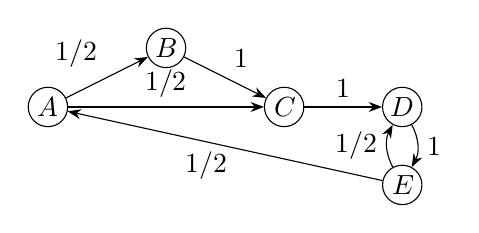
\begin{tikzpicture}[x=1.50cm,y=.60cm,>=Stealth,
  pgfnode/.style={circle,draw,inner sep=1pt,minimum size=5mm},every node/.style={font=\normalsize}]
\node[pgfnode] (A) at (0,0) {$A$};
\node[pgfnode] (B) at (1,1.25) {$B$};
\node[pgfnode] (C) at (2,0) {$C$};
\node[pgfnode] (D) at (3,0) {$D$};
\node[pgfnode] (E) at (3,-1.65) {$E$};
\draw[->] (A) -- (B) node[midway,above left] {$1/2$};
\draw[->] (A) -- (C) node[midway,above] {$1/2$};
\draw[->] (B) -- (C) node[midway,above right] {$1$};
\draw[->] (C) -- (D) node[midway,above] {$1$};
\draw[->] (D) to[bend left=28] node[midway,right] {$1$} (E);
\draw[->] (E) to[bend left=28] node[midway,left] {$1/2$} (D);
\draw[->] (E) -- (A) node[pos=.56,below] {$1/2$};
\end{tikzpicture}
\end{diagram}
Nhãn cạnh là phần điểm truyền đi. Cột $A$ có $1/2$ ở hàng $B,C$. Từ điểm ban đầu đều bằng 1, $C$ nhận $1/2$ từ $A$ và 1 từ $B$: $r_C^{(1)}=3/2$. Vòng sau $C$ nhận $(1/2)(1/2)+1/2=3/4$.
\end{example}

\ask{Pr16}{Pr16}{}
\original{DSA5101 Exam Practice Questions.pdf}{17}{53 503.890 542 756.890}
\answer{\maptag{answer:Pr16}}
\begin{guidesteps}[beginpenalty=10000]
\item \guidepart{(a)}Nhân ma trận theo thứ tự $H,L,R,S$: $M_0r=(1/5,2/5,1/5,0)^T$. Tổng chỉ $4/5$ vì cột $S$ bằng 0.
\item Nhân $\beta=1/2$ được $u=(1/10,1/5,1/10,0)^T$.
\end{guidesteps}
\begin{guidesteps}
\item \guidepart{(b)}Cộng các phần tử của $u$ được $2/5$. Chia phần hụt đều: mỗi nút nhận $(1-2/5)/4=3/20$.
\item Vậy $r'=(1/4,7/20,1/4,3/20)^T$, tổng bằng 1.
\end{guidesteps}
\begin{guidesteps}
\item \guidepart{(c)}Thay cột của nút cụt $S$ bằng $(1/4,1/4,1/4,1/4)^T$. Cộng teleport đều vẫn giữ nguyên cột này.
\item Tổng 1 chỉ kiểm tra bảo toàn khối lượng; để kiểm tra hội tụ, so $r'$ với $r$ hoặc kiểm tra phương trình điểm bất động.
\end{guidesteps}

\ask[A2-Q2]{P24-Q5}{P24-Q5 / A2-Q2}{}
\original{2425Sem1-DSA5101.pdf}{17}{53 466.890 542 750.890}
\original{2425Sem1-DSA5101.pdf}{17}{53 387.890 542 433.890}
\original{2425Sem1-DSA5101.pdf}{17}{53 347.890 542 375.890}
\original{2425Sem1-DSA5101.pdf}{17}{53 270.890 542 325.890}
\original{2425Sem1-DSA5101.pdf}{17}{53 165.890 542 237.890}
\answer{\maptag{answer:A2-Q2}\maptag{answer:P24-Q5}}
\begin{guidesteps}[beginpenalty=10000]
\item \guidepart{(a)}Đặt cột là nguồn và hàng là đích theo thứ tự $A,B,C,D,E$. Mỗi nguồn chia đều 1 cho các cạnh ra: $A,E$ chia đôi, $B,C,D$ truyền toàn bộ cho đích duy nhất.
\item Ghi các trọng số ở ô tương ứng và điền 0 ở các ô còn lại:
\[
M=\begin{pmatrix}0&0&0&0&1/2\\1/2&0&0&0&0\\1/2&1&0&0&0\\0&0&1&0&1/2\\0&0&0&1&0\end{pmatrix}.
\]
\end{guidesteps}
\begin{guidesteps}
\item \guidepart{(b)}Bắt đầu với $r^{(0)}=(1,1,1,1,1)^T$. Nhân $M$ một lần để được $r^{(1)}$, rồi dùng $r^{(1)}$ để tính $r^{(2)}$:
\[
\begin{aligned}
r^{(1)}&=(1/2,1/2,3/2,3/2,1)^T,\\
r^{(2)}&=(1/2,1/4,3/4,2,3/2)^T.
\end{aligned}
\]
\end{guidesteps}
\begin{guidesteps}
\item \guidepart{(c)}Giữ tổng điểm 5: nhân $r^{(1)}$ với 0.9 rồi cộng $0.1(5)(1/2,1/2,0,0,0)^T$. Được $(0.70,0.70,1.35,1.35,0.90)^T$.
\item Nêu mốc so sánh: so với vòng 1 không teleport, $A,B$ tăng; so với vectơ ban đầu, $C,D$ tăng.
\end{guidesteps}

\topic{teleport}{PageRank: teleport distributions \& convergence}
\key{Chọn phân phối $v$} PageRank thường dùng đều trên mọi nút. Topic-sensitive dùng đều trên tập chủ đề. Personalized có thể dồn toàn bộ xác suất vào một seed.

\key{Ba hiện tượng}
\begin{itemize}
\item Dead end: nút không có cạnh ra; nếu không sửa cột, tổng điểm bị hụt.
\item Spider trap: tập nút giữ điểm bên trong vì không có cạnh thoát. Teleport tới bên ngoài giúp điểm thoát.
\item Periodic walk: chẳng hạn chu trình hai nút có thể đổi chỗ điểm ở mỗi vòng dù vẫn có phân phối dừng.
\end{itemize}
\key{Hội tụ} Với $0<\beta<1$ và teleport dương trên mọi nút, ma trận chuyển sau sửa nút cụt có phân phối dừng duy nhất và lặp hội tụ. Nếu chỉ teleport vào một tập con, không mặc định mọi nút đều thông nhau.



\topic{trust}{TrustRank / spam mass}
\key{Khi dùng} Đề so PageRank thường $r$ với điểm tin cậy $t$, trong đó teleport chỉ ưu tiên các trang tin cậy. Giữ cùng đồ thị và quy ước chuẩn hóa khi so sánh.

\[
t=\beta Mt+(1-\beta)v_{\mathrm{trusted}},\qquad
\mathrm{SM}_i=\frac{r_i-t_i}{r_i}\quad(r_i>0).
\]
\key{Diễn giải} Nếu $r_i=0.2$ và $t_i=0.05$ thì spam mass bằng $0.75$. Giá trị cao cho biết phần lớn điểm không được giải thích bởi TrustRank; dùng để gắn cờ. Trang tin cậy có thể có spam mass âm.

\hard{P25-Q5}{Giải điểm cố định trên chu trình}
Trên chu trình $L$ nút với xác suất tiếp tục $\beta$ và teleport chỉ về nút 0, viết $r_j=\beta^j r_0$. Điểm về nút 0 gồm teleport và phần đi hết vòng: $r_0=(1-\beta)+\beta^Lr_0$. Với $L=3,\beta=3/5$, suy ra $r_0=(1-3/5)/(1-(3/5)^3)=25/49$, rồi nhân $3/5$ hai lần. Với $\beta=1$, công thức này không dùng được: phép lặp chỉ xoay vectơ. Điểm dừng đều tồn tại, nhưng toàn bộ dãy chỉ hội tụ nếu bắt đầu tại đó.

\ask{Pr18}{Pr18}{}
\original{DSA5101 Exam Practice Questions.pdf}{19}{53 599.890 542 784.890}
\answer{\maptag{answer:Pr18}}
\begin{guidesteps}[beginpenalty=10000]
\item \guidepart{(a)}Liệt kê nguồn vào $T$: $H$ có 2 cạnh ra, $F$ có 1. Cộng $\tfrac12(t_H/2+t_F)=2/21$.
\item $T$ không nhận teleport trực tiếp nhưng nhận điểm truyền qua các cạnh vào.
\end{guidesteps}
\begin{guidesteps}
\item \guidepart{(b)}Tính spam mass của $F$: $1-t_F/r_F=1-(1/21)/(2/7)=5/6>3/4$. Gắn cờ để kiểm tra; cờ không chứng minh spam.
\end{guidesteps}
\begin{guidesteps}
\item \guidepart{(c)}Chuyển $\tfrac14 r_T$ sang trái: $\tfrac34r_T=x+\tfrac3{16}$. Chia cho $3/4$ được $r_T=\tfrac43x+\tfrac14$.
\item Hệ số $4/3>1$ trước $x$ đo khuếch đại do điểm quay lại trong farm.
\end{guidesteps}

\ask{P25-Q5}{P25-Q5}{}
\original{2526Sem1-DSA5101.pdf}{15}{53 497.890 542 750.890}
\original{2526Sem1-DSA5101.pdf}{15}{53 372.890 542 407.890}
\original{2526Sem1-DSA5101.pdf}{15}{53 229.890 542 248.890}
\original{2526Sem1-DSA5101.pdf}{16}{53 719.890 542 738.890}
\original{2526Sem1-DSA5101.pdf}{16}{53 448.890 542 486.890}
\answer{\maptag{answer:P25-Q5}}
\begin{guidesteps}[beginpenalty=10000]
\item \guidepart{(a)}Theo cạnh có hướng, mỗi vòng chuyển $(a,b,c)$ thành $(c,a,b)$. Sau ba vòng trở lại điểm đầu.
\item Chu kỳ chỉ co thành điểm bất động khi $a=b=c$. Tổng bằng 1 nên chỉ hội tụ nếu bắt đầu tại $(1/3,1/3,1/3)$.
\end{guidesteps}
\begin{guidesteps}
\item \guidepart{(b)}Viết điểm vào mỗi nút bằng 0.6 lần điểm nút trước; chỉ $A$ nhận thêm teleport 0.4. Được $a=0.6c+0.4$, $b=0.6a$, $c=0.6b$.
\end{guidesteps}
\begin{guidesteps}
\item \guidepart{(c)}Thế từ $b$ vào $c$ được $c=0.36a$, rồi thế vào phương trình đầu: $a=0.216a+0.4$.
\item Giải và thế ngược: $(a,b,c)=(25/49,15/49,9/49)$; kiểm tra tổng bằng 1.
\end{guidesteps}
\begin{guidesteps}
\item \guidepart{(d)}Do chu trình đối xứng, PageRank dừng thường là $r_i=1/3$. Thế điểm tin cậy $t_i$ vào $1-t_i/r_i$.
\item Kết quả theo thứ tự $A,B,C$: $(-26/49,4/49,22/49)$. $A$ âm vì $t_A>1/3$.
\end{guidesteps}
\begin{guidesteps}
\item \guidepart{(e)}Chuẩn hóa phần điểm thiếu tin cậy theo tổng điểm của chính trang qua spam mass. Sau đó đặt ngưỡng để gắn cờ giá trị cao.
\item PageRank thấp riêng lẻ không nói trang có đáng tin hay không.
\end{guidesteps}

\topic{hits}{HITS (hubs and authorities)}
\key{Khi dùng} Muốn xếp hai vai trò: hub tốt trỏ tới nhiều authority tốt; authority tốt được hub tốt trỏ đến.

\key{Cách tính} Đặt ma trận kề $B$ có hàng là hub, cột là authority. Tính $h=Ba$ trước, sau đó dùng $h$ mới để tính $a'=B^Th$. Chuẩn hóa theo đề. Qua nhiều vòng, hướng của authority và hub tương ứng với vectơ riêng trội của $B^TB$ và $BB^T$.

\key{Bẫy} HITS cộng điểm qua mỗi cạnh mà không chia theo bậc ra như PageRank.

\ask{Pr17}{Pr17}{}
\original{DSA5101 Exam Practice Questions.pdf}{18}{53 640.890 542 784.890}
\answer{\maptag{answer:Pr17}}
\begin{guidesteps}[beginpenalty=10000]
\item \guidepart{(a)}Điền 1 ở mỗi liên kết từ hàng hub tới cột resource: $B=\bigl(\begin{smallmatrix}1&1&1\\1&1&0\\0&0&1\end{smallmatrix}\bigr)$.
\item Nhân $Ba^{(0)}$ với $a^{(0)}=(1,1,1)^T$, được $h=(3,2,1)^T$.
\end{guidesteps}
\begin{guidesteps}
\item \guidepart{(b)}Cộng điểm hub vào từng resource: $a'=B^Th=(3+2,3+2,3+1)^T=(5,5,4)^T$. Xếp $R_1=R_2>R_3$.
\end{guidesteps}
\begin{guidesteps}
\item \guidepart{(c)}Cùng indegree nhưng $R_1,R_2$ nhận từ $H_2$ có điểm cao hơn $H_3$ của $R_3$. HITS cộng cả điểm hub ở mỗi liên kết; PageRank chia điểm nguồn theo bậc ra.
\end{guidesteps}

\lecture{7}{Communities / graph clustering}

\topic{louvain}{Louvain / modularity}
\key{Khi dùng} Cần tìm phân hoạch toàn đồ thị theo modularity. Trong đồ thị vô hướng có $m$ cạnh, $e_C$ là số cạnh nội bộ của cụm $C$ đếm một lần và $\operatorname{vol}(C)=\sum_{v\in C}d_v$.
\[
Q=\sum_C\left[\frac{e_C}{m}-\left(\frac{\operatorname{vol}(C)}{2m}\right)^2\right].
\]
\steps{
\item Khởi tạo mỗi nút một cụm. Chuyển từng nút sang cụm lân cận cho mức tăng $Q$ tốt nhất nếu mức tăng dương.
\item Khi không còn cải thiện ở mức đang xét, gộp mỗi cụm thành một siêu nút, giữ đúng trọng số cạnh và self-loop rồi lặp.
}
\key{Tra ký hiệu} $\Sigma_{\rm in}=2e_C$ và $\Sigma_{\rm tot}=\operatorname{vol}(C)$ cho đồ thị vô hướng không trọng số. Louvain là heuristic; nếu chỉ quan tâm vùng quanh một seed, xem Local PPR.

\hard{P25-Q4}{Tách phần cạnh và phần thể tích trong modularity}
Nếu chuyển $i$ từ $A$ sang $B$, đặt $a=\operatorname{vol}(A)$ (gồm $i$), $b=\operatorname{vol}(B)$ và $k=d_i$. Gọi $k_{i,A},k_{i,B}$ là số cạnh từ $i$ tới phần còn lại của $A$ và tới $B$. Chỉ hai cụm đổi:
\[
\Delta Q=\frac{k_{i,B}-k_{i,A}}{m}
-\frac{(a-k)^2+(b+k)^2-a^2-b^2}{(2m)^2}.
\]
Trong \qlink{Pr20}{Pr20}, chuyển nút $3$ sang cụm $\{4\}$ với $m=5$, $a=b=k=2$, $k_{i,A}=0,k_{i,B}=1$: $\Delta Q=1/5-8/100=3/25$. Với vòng $K$ cụm đều nhau ở P25-Q4, nếu mỗi cụm có $e$ cạnh nội bộ và hai đầu cầu, thì $m=K(e+1)$, $\Sigma_{\rm in}=2e$, $\Sigma_{\rm tot}=2e+2$. Do đó $Q=e/(e+1)-1/K$; thế $e=N$ hoặc $e=\binom N2$.

\key{Kiểm tra khi co đồ thị} Với ma trận kề đối xứng có tổng hàng là bậc, đường chéo của siêu nút giữ $2e_C$; phần ngoài đường chéo đếm các cạnh nối hai cụm. Nhờ đó $\sum_{ij}B_{ij}=2m$ không đổi. Trong Pr20, hàng giữa của ma trận co là $(1,2,1)$: bậc $4$, trong đó $2$ đến từ một cạnh nội bộ. Xóa đường chéo sẽ làm sai cả thể tích và modularity.

\ask{Pr20}{Pr20}{}
\original{DSA5101 Exam Practice Questions.pdf}{21}{53 484.890 542 784.890}
\answer{\maptag{answer:Pr20}}
\begin{guidesteps}[beginpenalty=10000]
\item \guidepart{(a)}Sau khi ghép 3 vào cụm của 4, các cặp $(e,\mathrm{vol})$ là $(1,3),(1,4),(1,3)$. Thế vào $Q$: $2(1/5-9/100)+(1/5-16/100)=13/50$.
\item Trừ $7/50$ được gain $3/25>2/25$. Chọn ghép vào cụm 4.
\end{guidesteps}
\begin{guidesteps}
\item \guidepart{(b)}Cộng các hàng của ma trận gộp để có bậc $(3,4,3)$; chia tổng cho 2 được $m=5$.
\item Giữ đường chéo vì nó chứa hai lần trọng số cạnh nội bộ; bỏ nó sẽ làm sai bậc và modularity.
\end{guidesteps}
\begin{guidesteps}
\item \guidepart{(c)}Cả hai phép gộp kế tiếp đều giảm $Q$, nên thuật toán dừng. Nhưng $123|456$ có $Q=3/10>13/50$: điểm dừng không tối ưu toàn cục.
\end{guidesteps}

\ask{P25-Q4}{P25-Q4}{}
\original{2526Sem1-DSA5101.pdf}{12}{53 676.890 542 750.890}
\original{2526Sem1-DSA5101.pdf}{12}{53 467.890 542 642.890}
\original{2526Sem1-DSA5101.pdf}{12}{53 319.890 542 442.890}
\original{2526Sem1-DSA5101.pdf}{12}{53 232.890 542 251.890}
\original{2526Sem1-DSA5101.pdf}{12}{53 52.890 542 161.890}
\original{2526Sem1-DSA5101.pdf}{13}{53 678.890 542 743.890}
\original{2526Sem1-DSA5101.pdf}{13}{53 577.890 542 594.890}
\original{2526Sem1-DSA5101.pdf}{13}{53 419.890 542 495.890}
\original{2526Sem1-DSA5101.pdf}{13}{53 275.890 542 292.890}
\original{2526Sem1-DSA5101.pdf}{13}{53 131.890 542 149.890}
\original{2526Sem1-DSA5101.pdf}{14}{53 583.890 542 741.890}
\original{2526Sem1-DSA5101.pdf}{14}{53 460.890 542 481.890}
\original{2526Sem1-DSA5101.pdf}{14}{53 315.890 542 348.890}
\answer{\maptag{answer:P25-Q4}}
\begin{guidesteps}[beginpenalty=10000]
\item \guidepart{(a), (b)(i)}Đếm $e$ cạnh nội bộ mỗi cụm: $e=N$ cho chu trình, $e=N(N-1)/2$ cho clique. Có $K$ cầu nên $m=K(e+1)$.
\item Đếm cạnh nội bộ hai lần trong $\Sigma_{\rm in}=2e$; thêm hai đầu cầu được $\Sigma_{\rm tot}=2e+2$:
\begin{examtable}{@{}l c c c@{}}
\toprule
Cụm & $2m$ & $\Sigma_{\rm in}$ & $\Sigma_{\rm tot}$ \\
\midrule
Chu trình & $2K(N+1)$ & $2N$ & $2N+2$ \\
Clique & $K[N(N-1)+2]$ & $N(N-1)$ & $N(N-1)+2$ \\
\bottomrule
\end{examtable}
\end{guidesteps}
\begin{guidesteps}
\item \guidepart{(b)(ii)}Thế $\Sigma_{\rm tot}/(2m)=1/K$. Mỗi cụm góp $e/[K(e+1)]-1/K^2$ vào modularity. Cộng $K$ cụm rồi thế $e$:
\[
\begin{aligned}
Q_{\rm cycle}&=1-\frac{2}{2N+2}-\frac1K,\\
Q_{\rm clique}&=1-\frac{2}{N(N-1)+2}-\frac1K.
\end{aligned}
\]
\item So hai trường hợp: $N=3$ cho cùng cấu trúc; $N>3$ cho clique nhiều cạnh nội bộ hơn nhưng cùng số cầu, nên modularity cao hơn với phân hoạch đã cho.
\end{guidesteps}
\begin{guidesteps}
\item \guidepart{(c)}Đếm tất cả cạnh kề $A$: hai cạnh trong cụm gốc, một sang $H_1$. Vậy $(k_A,k_{A,\rm in})=(3,1)$ khi xét chuyển sang $H_1$.
\item Lặp lại cho $B$: có $N-1$ cạnh trong clique gốc và một sang $H_1$, nên $(k_B,k_{B,\rm in})=(N,1)$.
\end{guidesteps}
\begin{guidesteps}
\item \guidepart{(d)}Xác định phạm vi: cần phân hoạch toàn đồ thị, không có seed, thì chọn Louvain. Nếu tìm một cộng đồng quanh seed đã biết, chọn Local PPR.
\end{guidesteps}

\topic{ppr}{Local approximate PPR + conductance sweep}
\key{Khi dùng} Đề cho một seed $s$ và hỏi tìm cộng đồng cục bộ. Giữ hai vectơ: $r$ là điểm đã chốt, $q$ là điểm còn chờ lan truyền. Khởi tạo $q_s=1$, các phần tử còn lại bằng 0.
\steps{
\item Chọn nút $u$ có $q_u/d_u\ge\varepsilon$. Đặt $x=q_u$ trước khi cập nhật.
\item Với xác suất restart $1-\beta$ theo Practice, cộng $(1-\beta)x$ vào $r_u$, giữ $\beta x/2$ ở $q_u$ và cộng $\beta x/(2d_u)$ vào $q_v$ cho mỗi hàng xóm $v$.
\item Sắp nút theo điểm chuẩn hóa như đề cho. Với từng tiền tố $S$ hợp lệ, tính
\[
\phi(S)=\frac{\mathrm{cut}(S,\bar S)}
 {\min(\mathrm{vol}(S),\mathrm{vol}(\bar S))};
\]
chọn $S$ có conductance nhỏ nhất.
}
\key{Tự kiểm} Tổng $r+q$ vẫn bằng 1. Cut đếm cạnh băng qua; volume là tổng bậc, không phải số nút.

\hard{Pr19}{Cập nhật nhanh từng lát cắt trong sweep}
Khi thêm $u$ vào $S$, có $h$ cạnh nối $u$ với $S$ cũ. Những cạnh này biến từ cạnh cắt thành cạnh nội bộ; $d_u-h$ cạnh còn lại trở thành cạnh cắt. Vì vậy $\mathrm{cut}'=\mathrm{cut}+d_u-2h$ và $\mathrm{vol}'=\mathrm{vol}+d_u$. Trong Pr19, từ $S=\{A,C\}$ thêm $B$ có $d_B=h=2$, nên cut giảm từ $3$ xuống $1$, volume tăng từ $5$ lên $7$. Bỏ qua tập rỗng và toàn bộ đồ thị vì mẫu số bằng 0.

\begin{example}{Pr19}{Pr19(c) · Conductance: tìm điểm cắt bằng sweep}
\begin{diagram}
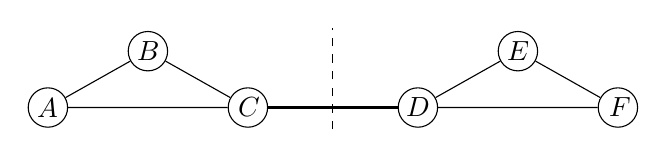
\begin{tikzpicture}[x=1.27cm,y=.53cm,every node/.style={font=\normalsize},
  sensor/.style={circle,draw,fill=white,inner sep=0pt,minimum size=5mm}]
\node[sensor] (A) at (0,0) {$A$};
\node[sensor] (B) at (1,1.35) {$B$};
\node[sensor] (C) at (2,0) {$C$};
\node[sensor] (D) at (3.7,0) {$D$};
\node[sensor] (E) at (4.7,1.35) {$E$};
\node[sensor] (F) at (5.7,0) {$F$};
\draw (A)--(B)--(C)--(A) (D)--(E)--(F)--(D);
\draw[very thick] (C)--(D);
\draw[dashed] (2.85,-.52)--(2.85,1.90);
\end{tikzpicture}
\end{diagram}
Theo thứ tự $A,C,B$, tập $\{A,C\}$ cắt 3 cạnh và có thể tích $2+3=5$, nên $\phi=3/5$. Thêm $B$ thì $AB$ và $BC$ thành cạnh nội bộ. Chỉ còn cắt $CD$; hai nửa đều có thể tích 7 nên $\phi=1/7$.
\end{example}

\ask{Pr19}{Pr19}{}
\original{DSA5101 Exam Practice Questions.pdf}{20}{53 544.890 542 756.890}
\answer{\maptag{answer:Pr19}}
\begin{guidesteps}[beginpenalty=10000]
\item \guidepart{(a)}Lấy $x=q_A=1$. Chuyển $(1-\beta)x=1/2$ vào $r_A$; giữ $\beta x/2=1/4$ ở $q_A$ và gửi $1/8$ cho mỗi láng giềng $B,C$.
\item Chia residual cho bậc: $1/8,1/16,1/24$. So với $1/20$: $A,B$ đủ điều kiện; chọn $A$ có tỉ số lớn nhất.
\end{guidesteps}
\begin{guidesteps}
\item \guidepart{(b)}Với $AC$, cạnh cắt là $AB,BC,CD$; volume $2+3=5$, nên $\phi=3/5$.
\item Với $ACB$, chỉ $CD$ cắt; volume 7, nên $\phi=1/7$. So cả singleton $A$ có $\phi=1$: chọn $ACB$.
\end{guidesteps}
\begin{guidesteps}
\item \guidepart{(c)}Cộng cả điểm và residual: $\sum_u(r_u+q_u)=1$. Một push chỉ đọc nút đang xử lý và các láng giềng, nên không cần quét đồ thị.
\end{guidesteps}

\topic{embedding}{Node embeddings: shallow encoding \& random walks}
\key{Ý chính} Mỗi nút $u$ được gán một vectơ học được $z_u$. Hai nút hay xuất hiện trong cửa sổ của cùng random walk nên có vectơ dễ dự đoán nhau, dù không có cạnh trực tiếp.

\steps{
\item Sinh các random walk; lấy các cặp nút trung tâm $u$ và nút ngữ cảnh $v$ trong cửa sổ. Giữ số lần cặp xuất hiện.
\item Học các vectơ bằng cách tăng xác suất của cặp quan sát:
\[
P(v\mid u)=\frac{\exp(z_v^Tz_u)}{\sum_{w\in V}\exp(z_w^Tz_u)}.
\]
Tương đương tối thiểu hóa tổng $-\log P(v\mid u)$ trên các cặp dương.
}
\key{Bẫy} Mẫu số softmax đi qua mọi nút. Bảng tra theo ID cần $O(d|V|)$ ô và không tự sinh vectơ cho nút chưa thấy.



\topic{node2vec}{DeepWalk vs node2vec (walk generation)}
\key{Phân biệt} DeepWalk đi ngẫu nhiên đều trên hàng xóm nếu cạnh không trọng số. node2vec còn xét nút ngay trước đó $t$ để quyết định bước tiếp từ $v$.

\key{Cách tính} Với ứng viên $x\in N(v)$, nhân trọng số cạnh $w_{vx}$ với hệ số dưới đây rồi chuẩn hóa trên toàn bộ hàng xóm của $v$:
\[
\alpha_{pq}(t,x)=
\begin{cases}
1/p & x=t \quad\text{(quay lại)},\\
1 & d(t,x)=1 \quad\text{(gần)},\\
1/q & d(t,x)=2 \quad\text{(đi xa)}.
\end{cases}
\]
\key{Ví dụ} $p=2,q=1/2$, mỗi loại một ứng viên không trọng số: điểm thô $(1/2,1,2)$, xác suất $(1/7,2/7,4/7)$. Đo $d(t,x)$ từ nút trước, không đo từ $v$. $q$ nhỏ thiên về đi xa; $q$ lớn thiên về quanh vùng hiện tại.



\topic{negatives}{Negative sampling for graph embeddings}
\key{Khi dùng} Muốn tránh tính mẫu số softmax trên mọi nút cho từng cặp. Cặp $(u,v)$ từ cửa sổ walk là dương; lấy $k$ mẫu nhiễu $n_j$ từ phân phối nền.
\[
\log\sigma(z_u^Tz_v)+\sum_{j=1}^k\log\sigma(-z_u^Tz_{n_j}),
\qquad \sigma(a)=\frac{1}{1+e^{-a}}.
\]
\key{Diễn giải} Tối đa hóa biểu thức để tăng tích vô hướng của cặp dương và giảm tích vô hướng của cặp nhiễu. Mỗi cặp tốn khoảng $O((k+1)d)$ thay vì $O(|V|d)$. Đây là mục tiêu huấn luyện khác full softmax.



\lecture{8}{Data streams}

\topic{fm}{Flajolet-Martin (FM): distinct count}
\key{Khi dùng} Ước lượng số ID khác nhau $F_0$ trên luồng. Mỗi ID lặp lại nhận cùng mã băm nên không làm thay đổi kết quả đã ghi cho ID đó.
\steps{
\item Đếm số bit 0 liên tiếp ở cuối mỗi mã băm. Lấy số lớn nhất $R$ cho mỗi hàm băm.
\item Ước lượng thô $2^R$. Với nhiều thanh ghi, lấy trung bình trong nhóm, rồi trung vị giữa các nhóm theo cách chia của đề.
\item Khi gộp hai monitor dùng cùng danh sách hash, lấy $\max$ theo từng thanh ghi trước khi đổi thành $2^R$.
}
\key{Bẫy} Một $R$ lớn hiếm gặp có thể kéo trung bình lên mạnh. $F_0$ không phải độ dài luồng.

\hard{P25-Q3}{Chứng minh cận dưới cho hash tốt nhất}
Để chứng minh ước lượng nhỏ nhất, tìm một tính chất đúng với mọi hash rồi cho một hash đạt cận. Với $h_i(x)=(x+i)\bmod 2^{16}$, cộng $i$ giữ hoặc đảo tính chẵn lẻ đồng loạt vì modulus chẵn. Hai đầu vào 1 và 10 luôn cho một giá trị chẵn, nên luôn có $R\ge1$. $h_0$ đạt $R=1$, vậy $2$ là cực tiểu. Nếu gặp mã 0, áp dụng quy ước độ dài bit của đề; không bỏ qua mã đó.

\begin{example}{P25-Q3}{P25-Q3(a,b) · Flajolet--Martin: đếm bit 0 ở cuối}
\begin{examtable}{@{}l c c c c c@{}}
\toprule
Hash & ID 1 & ID 5 & ID 10 & Các số bit 0 cuối & $2^R$ \\
\midrule
$h_0(x)=x$ & $0001$ & $0101$ & $1010$ & $(0,0,1)$ & 2 \\
$h_1(x)=x+1$ & $0010$ & $0110$ & $1011$ & $(1,1,0)$ & 2 \\
\bottomrule
\end{examtable}
Chỉ viết 4 bit thấp vì đủ để thấy bit 1 cuối trong các giá trị này. Cả hai hash đều có $R=1$: ước lượng thô là 2 dù thực tế có 3 ID phân biệt.
\end{example}

\ask{Pr24}{Pr24}{}
\original{DSA5101 Exam Practice Questions.pdf}{25}{53 599.890 542 784.890}
\answer{\maptag{answer:Pr24}}
\begin{guidesteps}[beginpenalty=10000]
\item \guidepart{(a)}Đếm bit 0 cuối của $12,10,7,6,3$: $(2,1,0,1,0)$. Lấy max $R_1=2$, nên $Z_1=4$; thực tế có 5 ID.
\item Gặp lại $A$ vẫn dùng hash 12, nên không tăng thanh ghi.
\end{guidesteps}
\begin{guidesteps}
\item \guidepart{(b)}Đổi từng thanh ghi sang $2^{R_j}$ được $(4,8,4,4,2,64)$. Trung bình theo cặp: $(6,4,33)$.
\item Lấy trung vị bằng 6; giá trị 64 chỉ kéo lệch một nhóm.
\end{guidesteps}
\begin{guidesteps}
\item \guidepart{(c)}Lấy max từng tọa độ của hai monitor, được $(2,3,2,2,1,6)$. Cùng ID cho cùng hash nên lấy max không đếm trùng.
\end{guidesteps}

\ask[A2-Q4]{P24-Q7}{P24-Q7(a,b) / A2-Q4(a,b)}{}
\original{2425Sem1-DSA5101.pdf}{19}{53 668.890 542 747.890}
\original{2425Sem1-DSA5101.pdf}{19}{53 567.890 542 649.890}
\answer{\maptag{answer:A2-Q4}\maptag{answer:A2-Q4ab}\maptag{answer:P24-Q7}\maptag{answer:P24-Q7ab}}
\begin{guidesteps}[beginpenalty=10000]
\item \guidepart{(a)}Liệt kê các giá trị khác nhau $1,\ldots,10$; tần suất khác nhau không ảnh hưởng $F_0$. Kết quả $F_0=10$.
\end{guidesteps}
\begin{guidesteps}
\item \guidepart{(b)}Với identity hash, đếm bit 0 ở cuối của $1,\ldots,10$: $(0,1,0,2,0,1,0,3,0,1)$.
\item Giá trị lớn nhất đến từ $8=1000_2$, nên $R=3$ và ước lượng $2^3=8$.
\end{guidesteps}

\ask{P25-Q3}{P25-Q3}{}
\original{2526Sem1-DSA5101.pdf}{5}{53 640.890 542 749.890}
\original{2526Sem1-DSA5101.pdf}{5}{53 523.890 542 543.890}
\original{2526Sem1-DSA5101.pdf}{5}{53 371.890 542 427.890}
\original{2526Sem1-DSA5101.pdf}{5}{53 180.890 542 244.890}
\answer{\maptag{answer:P25-Q3}}
\begin{guidesteps}[beginpenalty=10000]
\item \guidepart{(a)}Tính $h_0$ cho ba đầu vào, được $(1,5,10)$. Số bit 0 cuối là $(0,0,1)$; lấy max 1 rồi trả $2^1=2$.
\end{guidesteps}
\begin{guidesteps}
\item \guidepart{(b)}Tính $h_1$, được $(2,6,11)$. Số bit 0 cuối là $(1,1,0)$; lấy max 1 rồi trả $2^1=2$.
\end{guidesteps}
\begin{guidesteps}
\item \guidepart{(c)}Hai đầu vào 1 và 10 trái tính chẵn lẻ. Cộng cùng $i$ và lấy modulo chẵn vẫn có một mã chẵn, nên $R\ge1$.
\item Ở (a), $h_0$ cho $R=1$. Cận dưới đạt được, nên ước lượng nhỏ nhất là 2.
\end{guidesteps}
\begin{guidesteps}
\item \guidepart{(d)}Đổi từng thanh ghi thành $2^R$. Vì một $R$ lớn có thể kéo lệch trung bình chung, chia các ước lượng thành nhóm.
\item Lấy trung bình từng nhóm rồi lấy trung vị các trung bình đó.
\end{guidesteps}

\topic{ams}{AMS: frequency moments}
\key{Bài toán} Cho luồng $a_1,\ldots,a_n$ ($n\ge1$), với $m_i$ là số lần item $i$ xuất hiện và $d$ là số item phân biệt. Cần ước lượng $F_2=\sum_i m_i^2$ khi không đủ bộ nhớ để giữ tần suất của mọi item.

\begin{examtable}{@{}l l l@{}}
\toprule
& Đếm chính xác & AMS \\
\midrule
Lưu & Tần suất của mọi item & Item và bộ đếm của $k$ mẫu \\
Bộ nhớ & $O(d)$ & $O(k)$ \\
Kết quả & $F_2$ chính xác, tất định & $\widehat F_2$ ngẫu nhiên, không chệch \\
\bottomrule
\end{examtable}
\key{Một mẫu (slide 76)} Chọn đều một vị trí $t$ trong luồng. Lưu $\mathsf{X.el}=a_t$ và $\mathsf{X.val}=c$, số lần item đó xuất hiện từ vị trí $t$ đến cuối, tính cả $a_t$. Ước lượng là $Y=n(2c-1)$. Với $k$ mẫu, lấy trung bình các $Y$ để được $\widehat F_2$.

\key{Mã giả khi biết $n$}
\par\nopagebreak
\begin{tabular}{@{}l@{}}
Chọn đều $t\in\{1,\ldots,n\}$; đặt $\mathsf{X.el}=\varnothing$ và $c=0$. \\
Với mỗi cặp $(p,a_p)$ theo thứ tự của luồng: \\
\quad Nếu $p=t$: đặt $\mathsf{X.el}=a_p$ và $c=1$. \\
\quad Nếu $p>t$ và $a_p=\mathsf{X.el}$: tăng $c$ lên 1. \\
Trả $n(2c-1)$.
\end{tabular}\par
\key{Chi phí} Một mẫu dùng một lượt quét $O(n)$ thời gian và $O(1)$ bộ nhớ. Với $k$ mẫu, lưu $O(k)$ item và bộ đếm. Khi chưa biết $n$, dùng \hyperref[topic:reservoir]{reservoir sampling} để duy trì mẫu đều theo vị trí (slide 81). Khi nhận vị trí mới, tăng các bộ đếm đang giữ nếu item khớp; nếu vị trí mới được chọn, thay ô tương ứng bằng item mới và bộ đếm 1.

\key{Ví dụ: luồng $A,B,A,C,A,B$} Nếu chọn $t=3$, lưu item $A$ và đặt bộ đếm 1. Bảng cũng cho $c_t$ và $Y_t$ nếu bắt đầu ở bất kỳ vị trí $t$ nào.
\begin{examtable}{@{}c c c c l@{}}
\toprule
$t$ & $a_t$ & $c_t$ & $Y_t=6(2c_t-1)$ & Cập nhật khi chọn $t=3$ \\
\midrule
1 & $A$ & 3 & 30 & Chưa bắt đầu \\
2 & $B$ & 2 & 18 & Chưa bắt đầu \\
3 & $A$ & 2 & 18 & Khởi tạo: $c=1$ \\
4 & $C$ & 1 & 6  & Giữ $c=1$ \\
5 & $A$ & 1 & 6  & Tăng lên $c=2$ \\
6 & $B$ & 1 & 6  & Giữ $c=2$ \\
\bottomrule
\end{examtable}
Mẫu ở $t=3$ cho $Y=6(2\cdot2-1)=18$, còn giá trị chính xác là $3^2+2^2+1^2=14$. Trung bình qua cả sáu điểm bắt đầu là $(30+18+18+6+6+6)/6=14$.

\key{Vì sao không chệch (slides 77--78)} Nếu item $i$ xuất hiện $m_i$ lần, chọn từ lần đầu đến lần cuối cho các giá trị $c=m_i,m_i-1,\ldots,1$. Vì $2c-1=c^2-(c-1)^2$, tổng $1+3+\cdots+(2m_i-1)$ bằng $m_i^2$. Gom các vị trí theo item:
\[
\begin{aligned}
\mathbb E[Y]
  &=\frac1n\sum_{t=1}^n n(2c_t-1)\\
  &=\sum_i\sum_{c=1}^{m_i}(2c-1)
   =\sum_i m_i^2=F_2.
\end{aligned}
\]
Cùng lập luận cho moment bậc $r$: dùng $Y_r=n[c^r-(c-1)^r]$ để ước lượng $F_r=\sum_i m_i^r$. Bậc $1$ cho $F_1=n$.

\key{Tự kiểm trước khi thi}
\par\nopagebreak
\begin{examtable}{@{}p{.76\linewidth}l@{}}
\toprule
Phát biểu & Đúng/Sai \\
\midrule
AMS luôn trả đúng $F_2$. & Sai \\
$\mathbb E[\widehat F_2]=F_2$. & Đúng \\
$c$ luôn bằng tần suất của item trong cả luồng. & Sai \\
Chọn đều item phân biệt luôn tương đương chọn đều vị trí. & Sai \\
Mẫu tại vị trí đầu có thể cho $Y>F_2$. & Đúng \\
\bottomrule
\end{examtable}
Kỳ vọng xét qua các lần lấy mẫu ngẫu nhiên; một lần chạy không bắt buộc cho kết quả đúng. Chẳng hạn vị trí đầu của luồng trên cho 30. Chọn đều vị trí lấy được item $i$ với xác suất $m_i/n$, nên nói chung không thể thay bằng chọn đều trên các item phân biệt.

\hard{P24-Q7cd}{Phân biệt một mẫu với trung bình qua mọi vị trí}
Nếu đề yêu cầu dùng mỗi vị trí đúng một lần thì trung bình bằng $F_2$ một cách tất định, theo phép tính kỳ vọng ở trên. Trong P24-Q7/A2-Q4, $n=55$: theo thứ tự liệt kê, mẫu đầu cho 55, còn dùng cả 55 vị trí cho 385.

\begin{example}{Pr25}{Pr25(a) · AMS: cùng một luồng, hai vị trí lấy mẫu}
\begin{examtable}{@{}c l c c@{}}
\toprule
Vị trí bắt đầu & ID và vị trí lặp trong hậu tố & $c$ & $9(2c-1)$ \\
\midrule
1 & $R$ tại $1,3,6,9$ & 4 & 63 \\
2 & $F$ tại $2,5$ & 2 & 27 \\
\bottomrule
\end{examtable}
Lấy trung bình hai ước lượng được 45. Moment thực là $4^2+2^2+2^2+1^2=25$: một mẫu cụ thể có thể cho kết quả khác giá trị thực.
\end{example}

\ask{Pr25}{Pr25}{}
\original{DSA5101 Exam Practice Questions.pdf}{26}{53 559.890 542 784.890}
\answer{\maptag{answer:Pr25}}
\begin{guidesteps}[beginpenalty=10000]
\item \guidepart{(a)}Thế hai suffix count 4 và 2 vào $Y_2=9(2c-1)$: lần lượt được 63 và 27.
\item Lấy trung bình $(63+27)/2=45$. Một lần lấy mẫu có thể lệch khỏi $F_2=16+4+4+1=25$.
\end{guidesteps}
\begin{guidesteps}
\item \guidepart{(b)}Phát hiện thứ 10 là $R$: tăng bộ đếm ở ô 1 lên 5. $J_{10}=2$ thay ô 2 bằng $(10,R,1)$.
\item Hai ô cuối là $(1,R,5)$ và $(10,R,1)$; lấy trung bình $[10(9)+10(1)]/2=50$. Giữ hai bộ đếm vì chúng bắt đầu ở hai vị trí khác nhau.
\end{guidesteps}
\begin{guidesteps}
\item \guidepart{(c)}Thế $n=10,c=2$: $Y_3=10(2^3-1^3)=70$.
\item Dùng suffix count để các lần xuất hiện của một item lần lượt cho $m,m-1,\ldots,1$. Dùng tần suất toàn luồng sẽ lặp cùng $m$ và mất tổng triệt tiêu.
\end{guidesteps}

\ask[A2-Q4cd]{P24-Q7cd}{P24-Q7(c,d) / A2-Q4(c,d)}{Dữ kiện chung: \hyperref[question:P24-Q7]{[P24-Q7]}}
\original{2425Sem1-DSA5101.pdf}{19}{53 433.890 542 489.890}
\original{2425Sem1-DSA5101.pdf}{19}{53 267.890 542 354.890}
\original{2425Sem1-DSA5101.pdf}{19}{53 127.890 542 194.890}
\answer{\maptag{answer:A2-Q4cd}\maptag{answer:P24-Q7cd}}
\begin{guidesteps}[beginpenalty=10000]
\item \guidepart{(c)}Bình phương tần suất của từng giá trị rồi cộng: $F_2=1^2+\cdots+10^2=385$.
\end{guidesteps}
\begin{guidesteps}
\item \guidepart{(d)(i)}Tính độ dài $n=1+\cdots+10=55$. Theo thứ tự liệt kê, item đầu là 1 và chỉ xuất hiện một lần nên $c=1$.
\item Thế $Y=55(2c-1)=55$. Nếu không cố định thứ tự và luồng bắt đầu bằng $j$, dùng $c=j$, cho $55(2j-1)$.
\end{guidesteps}
\begin{guidesteps}
\item \guidepart{(d)(ii)}Gom các vị trí theo giá trị $j$. Các suffix count là $j,j-1,\ldots,1$, nên tổng $2c-1$ của nhóm là $j^2$.
\item Trong trung bình qua 55 vị trí, hệ số 55 triệt với phép chia 55. Cộng $j^2$ cho tất cả nhóm được 385 với mọi thứ tự.
\end{guidesteps}

\topic{dgim}{DGIM: sliding-window bit counts}
\key{Khi dùng} Đếm xấp xỉ số bit 1 trong $N$ vị trí gần nhất. Bucket cỡ $2^j$ chứa $2^j$ bit 1; timestamp là vị trí bit 1 mới nhất trong bucket.
\steps{
\item Khi đến vị trí $t$, xóa bucket có timestamp $\le t-N$.
\item Nếu bit đến là 1, thêm bucket cỡ 1. Khi có ba bucket cùng cỡ, gộp hai bucket cũ nhất và giữ timestamp mới hơn trong hai bucket. Lặp nếu tràn ở cỡ lớn hơn.
\item Khi hỏi $k$ vị trí cuối, bỏ bucket kết thúc trước cửa sổ truy vấn. Cộng đủ các bucket mới hơn và nửa bucket cũ nhất còn lại. Nếu không còn bucket, trả 0.
}
\key{Sai số} Nếu bucket cũ nhất có $2^j$ bit 1, phần sai lệch tối đa là $2^{j-1}$. Có ít nhất một bit 1 từ bucket này và ít nhất $2^j-1$ bit 1 từ các cỡ nhỏ hơn, nên sai số tương đối tối đa $50\%$ trong mô hình chuẩn. Lưu $O(\log^2N)$ bit cho $O(\log N)$ bucket và timestamp.

\hard{P24-Q6}{Ba cận khác nhau cho cửa sổ 500 bit}
Để tạo bucket cỡ $2b$, phải có đồng thời ba bucket cỡ $b$. Sau timestamp của bucket cũ nhất có ít nhất $2b$ bit 1 ở hai bucket mới hơn; vì bucket cũ nhất còn sống, $2b\le N-1$. Với $N=500$ không thể tạo cỡ 512, còn cỡ 256 đạt được qua 511 bit 1 liên tiếp. Cận nửa bucket là $256/2=128$; với cửa sổ này, ý (b) dưới đây chứng minh cận chặt là 127. Nếu cả 500 bit đều là 1, các cỡ $1$ đến $64$ chứa tối đa $2(1+2+4+\cdots+64)=254$ bit, nên cỡ lớn nhất phải ít nhất 128. Để chứng minh đạt cận dưới, chạy từ rỗng với đúng 500 bit 1: hai bucket cỡ 128, không có bucket cỡ 256.

\begin{example}{Pr22}{Pr22(a,b) · DGIM: xóa, thêm, gộp rồi truy vấn}
\begin{examtable}{@{}c l l@{}}
\toprule
$t$ & Thao tác & Bucket $(\text{cỡ},\text{timestamp})$, cũ trước \\
\midrule
13 & Trạng thái ban đầu & $(4,4), (2,10), (1,11), (1,13)$ \\
14 & Bit 0; hết hạn $(4,4)$ & $(2,10), (1,11), (1,13)$ \\
15 & Thêm $(1,15)$ & $(2,10), (1,11), (1,13), (1,15)$ \\
15 & Gộp hai bucket 1 cũ nhất & $(2,10), (2,13), (1,15)$ \\
\bottomrule
\end{examtable}
Hỏi 6 vị trí cuối ($10$ đến $15$): tính nửa bucket $(2,10)$, cộng trọn hai bucket mới hơn, được $2/2+2+1=4$.
\end{example}

\ask{Pr22}{Pr22}{}
\original{DSA5101 Exam Practice Questions.pdf}{23}{53 568.890 542 784.890}
\answer{\maptag{answer:Pr22}}
\begin{guidesteps}[beginpenalty=10000]
\item \guidepart{(a)}Ở $n=14$, loại $(4,4)$ vì $4\le14-10$; bit mới là 0. Còn $(2,10),(1,11),(1,13)$.
\item Ở $n=15$, thêm $(1,15)$. Gộp hai bucket cỡ 1 cũ nhất thành $(2,13)$, được $(2,10),(2,13),(1,15)$.
\end{guidesteps}
\begin{guidesteps}
\item \guidepart{(b)}Chọn bucket có timestamp từ 10 đến 15. Lấy nửa bucket cũ nhất và cộng nguyên các bucket mới hơn: $2/2+2+1=4$.
\item Đếm trực tiếp sáu bit cũng được 4; sự trùng nhau ở đây không bảo đảm DGIM luôn đúng.
\end{guidesteps}
\begin{guidesteps}
\item \guidepart{(c)}Nhân số đếm với trọng số bit $2^j$ rồi cộng: $\hat S=4+2(3/2)+4(3/2)=13$.
\item So với tổng đúng 16: sai số đến từ các ước lượng từng vị trí bit.
\end{guidesteps}

\ask[A2-Q3]{P24-Q6}{P24-Q6 / A2-Q3}{}
\original{2425Sem1-DSA5101.pdf}{18}{53 692.890 542 747.890}
\original{2425Sem1-DSA5101.pdf}{18}{53 428.890 542 544.890}
\original{2425Sem1-DSA5101.pdf}{18}{53 198.890 542 268.890}
\answer{\maptag{answer:A2-Q3}\maptag{answer:P24-Q6}}
\begin{guidesteps}[beginpenalty=10000]
\item \guidepart{(a)}Thử tạo bucket 512: cần ba bucket 256. Chỉ hai bucket mới đã có 512 bit 1 sau timestamp của bucket cũ nhất, nên bucket cũ đã hết hạn trong cửa sổ 500.
\item Chạy 511 bit 1 liên tiếp có bucket cỡ 256. Kết luận: cỡ lớn nhất là 256.
\end{guidesteps}
\begin{guidesteps}
\item \guidepart{(b)}Khi bucket biên cỡ 256, các bucket mới hơn có ít nhất một bucket mỗi cỡ $1,2,4,\ldots,128$, tổng ít nhất 255. Vì còn ít nhất 1 bit của bucket biên, số bit thực $x$ nằm trong $[1,245]$.
\item DGIM dùng 128 thay cho $x$. Sai số lớn nhất trên đoạn là $\max(128-1,245-128)=127$. Bucket nhỏ hơn có cận nửa bucket tối đa 64.
\item Dùng 511 bit 1 rồi 244 bit 0: đầu cửa sổ trùng timestamp của bucket 256, nên $x=1$ và đạt 127. Cận tổng quát 128 vẫn đúng nhưng không chặt.
\end{guidesteps}
\begin{guidesteps}
\item \guidepart{(c)}Nếu cỡ lớn nhất chỉ là 64, hai bucket mỗi cỡ chứa tối đa $2(1+2+\cdots+64)=254$ bit 1, không đủ cho 500 bit 1.
\item Từ rỗng chèn đúng 500 bit 1: có hai bucket cỡ 128, không có bucket lớn hơn. Kết luận: cỡ lớn nhất tối thiểu là 128.
\end{guidesteps}

\topic{bloom}{Bloom filter: approximate membership}
\key{Khi dùng} Hỏi một khóa đã từng xuất hiện hay chưa mà không giữ danh sách đầy đủ.
\steps{
\item Khi thêm khóa, bật $k$ vị trí do các hàm băm chỉ định trong cùng mảng $m$ bit.
\item Khi hỏi khóa, gặp ít nhất một bit 0 thì chắc chắn vắng. Nếu cả $k$ bit bằng 1 thì khóa có thể có mặt.
\item Với $n$ khóa đã thêm, dùng
\[
\Pr(\mathrm{FP})\approx(1-e^{-kn/m})^k,\qquad
k^*\approx(m/n)\ln2.
\]
So hai số nguyên lân cận $k^*$, với $k\ge1$.
}
\key{Bẫy} Có sai dương do khóa khác bật trùng bit. Với bộ lọc chuẩn không xóa bit và cùng các hàm băm, không có sai âm.

\hard{P25-Q6}{Giải ngược số bit, rồi tối ưu số hash nguyên}
Với một hash và $n$ khóa, yêu cầu $1-e^{-n/m}\le\alpha$ tương đương $m\ge n/[-\ln(1-\alpha)]$. Lấy trần để không vượt xác suất đích. Với $n=5000,\alpha=0.1$, mẫu số $-\ln(0.9)$ cho $m=47457$. Giữ $m$ và tìm $k^*\approx6.58$, rồi thế lại cả hai số nguyên: $f(6)\approx0.01058$, $f(7)\approx0.01052$, nên chọn 7. Không làm tròn mặc định: \qlink{Pr23}{Pr23(c)} là trường hợp so trực tiếp hai giá trị hàm.

\begin{example}{Pr23}{Pr23(a,b) · Bloom filter: một bit 0 đủ để loại}
\begin{diagram}
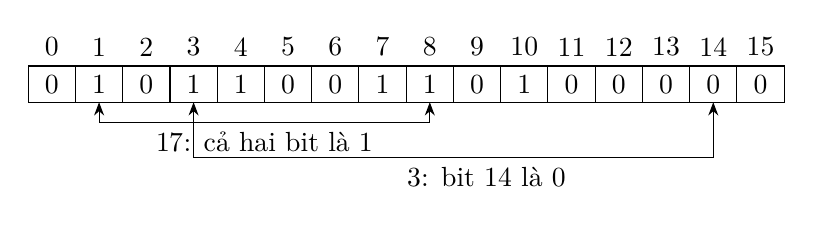
\begin{tikzpicture}[x=.60cm,y=.46cm,>=Stealth,every node/.style={font=\normalsize}]
\foreach \bit [count=\i from 0] in {0,1,0,1,1,0,0,1,1,0,1,0,0,0,0,0}{
  \draw (\i,0) rectangle ++(1,1);
  \node[above] at (\i+.5,1) {\i};
  \node at (\i+.5,.5) {\bit};
}
\draw[<-] (1.5,0)--(1.5,-.55)--(5,-.55);
\draw[->] (5,-.55)--(8.5,-.55)--(8.5,0);
\node[below] at (5,-.55) {$17$: cả hai bit là 1};
\draw[<-] (3.5,0)--(3.5,-1.53)--(9.7,-1.53);
\draw[->] (9.7,-1.53)--(14.5,-1.53)--(14.5,0);
\node[below] at (9.7,-1.53) {$3$: bit 14 là 0};
\end{tikzpicture}
\end{diagram}
Sau khi chèn $1,4,7,10$, truy vấn $17$ đọc $(1,8)$ và báo nhầm có mặt. Truy vấn $3$ đọc $(3,14)$ và kết luận chắc chắn vắng.
\end{example}

\ask{Pr23}{Pr23}{}
\original{DSA5101 Exam Practice Questions.pdf}{24}{53 552.890 542 784.890}
\answer{\maptag{answer:Pr23}}
\begin{guidesteps}[beginpenalty=10000]
\item \guidepart{(a)}Lấy hợp các vị trí hash đã cho: $\{1,3,4,7,8,10\}$. Đặt lại một bit đang là 1 không đổi trạng thái.
\end{guidesteps}
\begin{guidesteps}
\item \guidepart{(b)}ID 17 đọc $(1,8)$ đều là 1: báo có thể có, nhưng 17 chưa chèn nên dương giả.
\item ID 3 đọc $(3,14)$ có bit 14 bằng 0: báo không có. ID 3 thật sự vắng nên âm đúng.
\end{guidesteps}
\begin{guidesteps}
\item \guidepart{(c)}So hai số nguyên khả thi: $0.3935<0.3996$, chọn 1 hash. Điểm cực tiểu liên tục $1.386$ không bắt buộc làm tròn lên.
\item Nhân xác suất với 200 truy vấn vắng: số dương giả kỳ vọng $78.7$, khoảng 79.
\end{guidesteps}

\ask{P25-Q6}{P25-Q6}{}
\original{2526Sem1-DSA5101.pdf}{17}{53 604.890 542 750.890}
\original{2526Sem1-DSA5101.pdf}{17}{53 450.890 542 486.890}
\original{2526Sem1-DSA5101.pdf}{17}{53 218.890 542 258.890}
\answer{\maptag{answer:P25-Q6}}
\begin{guidesteps}[beginpenalty=10000]
\item \guidepart{(a)}Với một hash, áp dụng xấp xỉ $p_{\rm FP}\approx1-e^{-5000/m}$. Đặt giá trị này $\le0.1$ rồi giải $m\ge-5000/\ln(0.9)\approx47456.108$.
\item Làm tròn lên theo xấp xỉ của đề: 47457 bit.
\end{guidesteps}
\begin{guidesteps}
\item \guidepart{(b)}Chèn: dùng $k$ hash độc lập và bật tất cả vị trí trong cùng mảng. Truy vấn: nếu có bit 0 thì báo vắng; chỉ khi cả $k$ bit bằng 1 mới báo có thể có.
\end{guidesteps}
\begin{guidesteps}
\item \guidepart{(c)}Tính cực tiểu liên tục $k^*\approx(m/5000)\ln2\approx6.58$. Thử hai số nguyên kề $6,7$ trong $(1-e^{-5000k/m})^k$.
\item So $0.01058$ với $0.01052$: chọn 7 hash, xác suất dương giả khoảng $1.052\%$.
\end{guidesteps}

\topic{reservoir}{Reservoir / key sampling}
\key{Khi dùng} Cần lấy đúng $k$ bản ghi ngẫu nhiên từ luồng chưa biết độ dài.
\steps{
\item Lưu $k$ bản ghi đầu tiên vào $k$ ô.
\item Khi bản ghi thứ $n>k$ đến, rút đều $J$ từ 1 đến $n$. Nếu $J\le k$, thay ô $J$ bằng bản ghi mới.
}
\key{Tự kiểm} Sau $n$ bản ghi, mỗi bản ghi có xác suất nằm trong mẫu là $k/n$. Bản ghi cũ có xác suất sống qua bước $n$ là $(n-1)/n$, nếu trước đó đang nằm trong mẫu.

\key{Phân biệt} Key sampling băm theo ID người dùng nên giữ cả lịch sử của user được chọn; số bản ghi lưu có thể tăng theo luồng.

\ask{Pr21}{Pr21}{}
\original{DSA5101 Exam Practice Questions.pdf}{22}{53 491.890 542 756.890}
\answer{\maptag{answer:Pr21}}
\begin{guidesteps}[beginpenalty=10000]
\item \guidepart{(a)}Từ $(6,4,3)$, $J_7=3$ thay ô 3 bằng 7: $(6,4,7)$. $J_8=2$ thay ô 2 bằng 8: $(6,8,7)$.
\end{guidesteps}
\begin{guidesteps}
\item \guidepart{(b)}Bản ghi đã lưu chỉ mất nếu bốc đúng ô của nó: xác suất sống $7/8$. Vậy xác suất có mặt sau lượt 8 là $(3/7)(7/8)=3/8$.
\item Bản ghi mới được nhận nếu bốc 1, 2 hoặc 3, cũng có xác suất $3/8$.
\end{guidesteps}
\begin{guidesteps}
\item \guidepart{(c)}Vì $h(A)=1$, giữ các vị trí $1,3,5,8$. Theo hàng query của đề: ba $x$, một $w$. Reservoir $(6,8,7)$ chỉ giữ vị trí 8 của $A$.
\item Hash theo user giữ trọn lịch sử của user được chọn, nhưng số bản ghi có thể tăng theo luồng.
\end{guidesteps}

\topic{decay}{Decaying windows}
\key{Khi dùng} Đếm mức độ gần đây; mỗi bước thời gian làm điểm cũ giảm một nửa. Sự kiện loại $x$ ở bước $i$ đóng góp $2^{-(t-i)}$ vào điểm ở bước $t$.
\steps{
\item Chia đôi mọi điểm đang lưu, rồi cộng 1 cho loại vừa xuất hiện.
\item Nếu đề dùng pruning, xóa các loại có điểm dưới $\tau$ theo đúng dấu bất đẳng thức đề cho. Khi loại đó xuất hiện lại, cộng vào điểm đang lưu (hoặc 0 nếu đã xóa).
}
\key{Bẫy} Pruning mất phần lịch sử đã xóa nên có thể bỏ lỡ cảnh báo. Tổng trọng số không vượt 2; nếu giữ điểm $\ge\tau>0$, số mục không vượt $2/\tau$.

\ask{Pr26}{Pr26}{}
\original{DSA5101 Exam Practice Questions.pdf}{27}{53 580.890 542 784.890}
\answer{\maptag{answer:Pr26}}
\begin{guidesteps}[beginpenalty=10000]
\item \guidepart{(a)}Khi $E$ đến, chia đôi thành $\{A:1/4,D:1/2\}$, thêm $E:1$ rồi xóa $A$. Còn $\{D:1/2,E:1\}$.
\item Khi $A$ đến, chia đôi, thêm $A:1$ rồi xóa $D$ có điểm $1/4$. Còn $\{E:1/2,A:1\}$.
\end{guidesteps}
\begin{guidesteps}
\item \guidepart{(b)}So với ngưỡng $9/8$: điểm lưu $1$ không báo, còn $293/256>9/8$ có báo. Xóa sớm làm mất đóng góp quá khứ của $A$, gây âm giả.
\end{guidesteps}
\begin{guidesteps}
\item \guidepart{(c)}Tổng điểm tối đa 2, mỗi mục còn lại ít nhất $1/2$, nên số mục tối đa $2/(1/2)=4$.
\item Decay giảm dần trọng số theo tuổi; cửa sổ cố định giữ trọng số của các lượt trong cửa sổ rồi loại hẳn khi ra ngoài.
\end{guidesteps}

\lecture{9}{Online matching, BALANCE \& bandits}

\topic{matching}{Online bipartite matching}
\key{Khi dùng} Job đến lần lượt, mỗi server nhận tối đa một job và quyết định không được đổi lại.
\steps{
\item Xét danh sách hàng xóm của job vừa đến. Ghép với một server hợp lệ còn rảnh theo quy tắc đề; nếu không có thì bỏ qua.
\item Tính $\mathrm{ALG}/\mathrm{OPT}$, với OPT được biết cả chuỗi đến. Để tìm OPT, cho phép chọn lại từ đầu thay vì sửa lời giải greedy.
}
\key{Bảo đảm $1/2$} Matching greedy là maximal: không còn cạnh nối hai đầu mút chưa ghép. Mỗi cạnh OPT chạm ít nhất một cạnh greedy, và mỗi cạnh greedy chỉ có thể chạm tối đa hai cạnh OPT. Vì vậy $\mathrm{OPT}\le2\,\mathrm{ALG}$. Tỷ lệ của một ví dụ không phải cận cho mọi đầu vào.

\ask{Pr27}{Pr27}{}
\original{DSA5101 Exam Practice Questions.pdf}{28}{53 530.890 542 756.890}
\answer{\maptag{answer:Pr27}}
\begin{guidesteps}[beginpenalty=10000]
\item \guidepart{(a)}Chọn server khả dụng có chỉ số nhỏ nhất: $J_1\to S_1$, $J_2\to S_2$. $J_3$ bị loại vì chỉ dùng được $S_1$.
\item $J_4\to S_3$. Tổng cộng ghép 3 job.
\end{guidesteps}
\begin{guidesteps}
\item \guidepart{(b)}Ghép offline $J_1\to S_2,J_2\to S_3,J_3\to S_1,J_4\to S_4$. Cả bốn job đều hợp lệ và mỗi server dùng một lần, nên OPT bằng 4.
\item Tỉ lệ trên dữ liệu này là $3/4$.
\end{guidesteps}
\begin{guidesteps}
\item \guidepart{(c)}Quyết định online không thể hủy, nên không dời $J_1$ để nhường chỗ. Tỉ lệ một trường hợp không chứng minh cận cho mọi thứ tự đến.
\end{guidesteps}

\topic{balance}{BALANCE (unit bids / budgets)}
\key{Khi dùng} Mỗi query mang lại 1 đơn vị doanh thu. Chọn một advertiser đủ điều kiện có ngân sách còn lại lớn nhất, trừ 1 và chuyển sang query tiếp theo. Nếu không có advertiser phù hợp còn ngân sách, bỏ qua.

\key{Tính trên giấy} Viết vectơ ngân sách sau từng lượt; tuân thủ cách phá hòa. Nếu đề hỏi guaranteed optimal, tất cả cách phá hòa hợp lệ đều phải đạt OPT; chỉ cần tìm một nhánh thất bại để trả lời No.

\key{Bảo đảm theo mô hình} Hai advertiser cùng ngân sách $B$ chẵn, OPT phục vụ $2B$: BALANCE phục vụ ít nhất $3B/2$. Nếu còn query bị bỏ, ít nhất một bên đã hết ngân sách. Gọi $A$ là bên còn tiền. Cả $B$ query OPT giao cho $A$ đều được BALANCE phục vụ vì $A$ chưa bao giờ hết tiền. Nếu $A$ nhận ít nhất $B/2$ query thì đạt cận. Nếu hơn $B/2$ query đó sang bên kia, ở lần chuyển thứ $B/2+1$, bên kia còn tối đa $B/2$ ngân sách. Quy tắc chọn bên còn nhiều tiền hơn cho thấy $A$ cũng chỉ còn tối đa $B/2$. Lập luận với $B$ lẻ cho cận $\lfloor3B/2\rfloor$.

\key{Ví dụ} Với $B=4$, bốn query đầu cả hai đều nhận được, bốn query sau chỉ một bên nhận được: BALANCE đạt 6, OPT đạt 8. Trong mô hình nhiều advertiser của lecture, cận $1-1/e$ được suy ra từ phần ngân sách còn lại khi các bên lần lượt cạn.

\hard{A2-Q5}{Chứng minh tối ưu với mọi cách phá hòa}
Lập các trạng thái $(a,b)$ sau từng query; ở lượt hòa giữ cả hai nhánh và gộp trạng thái trùng. Tổng đã phục vụ bằng $2B-a-b$ ở mọi trạng thái. Tìm OPT bằng một cận (số query, tổng ngân sách hoặc số query chỉ một bên nhận được) cộng một lịch đạt cận. Với $yzyy$ trong A2-Q5(d), có 3 query $y$ chỉ $A$ nhận và $A$ có 2 đơn vị; OPT tối đa $2+1=3$. BALANCE phục vụ đúng hai $y$ và một $z$, nên đạt OPT dù không phục vụ hết.

\begin{example}{A2-Q5}{A2-Q5(c) · BALANCE: hai cách phá hòa, hai kết quả}
\begin{examtable}{@{}l c l l@{}}
\toprule
Query & Chọn & Ngân sách còn $(A,B)$ & Lý do \\
\midrule
$x$ & $A$ & $(1,2)$ & Hòa ở $(2,2)$ \\
$y$ & $A$ & $(0,2)$ & Chỉ $A$ đủ điều kiện \\
$x$ & $B$ & $(0,1)$ & $A$ hết tiền \\
$z$ & $B$ & $(0,0)$ & Chỉ $B$ đủ điều kiện \\
\bottomrule
\end{examtable}
Nhánh trên phục vụ đủ 4 query. Nếu $x$ đầu tiên sang $B$, sau $y$ còn $(1,1)$: chọn $B$ khi hòa ở $x$ thứ hai sẽ hết tiền cho $z$. Có nhánh chỉ phục vụ 3, nên đáp án là No.
\end{example}

\ask{Pr28}{Pr28}{}
\original{DSA5101 Exam Practice Questions.pdf}{29}{53 491.890 542 784.890}
\answer{\maptag{answer:Pr28}}
\begin{guidesteps}[beginpenalty=10000]
\item \guidepart{(a)}So ngân sách của $B,D$ ở lượt $v$ đầu: $D$ còn 2, nên chọn $D$. Còn $(1,1,1,1)$, doanh thu 4.
\item Lượt $v$ sau hòa giữa $B,D$; chọn $B$ theo bảng chữ cái. Còn $(1,0,1,1)$, doanh thu 5.
\end{guidesteps}
\begin{guidesteps}
\item \guidepart{(b)}Từ $(1,0,1,0)$, lượt $w$ đầu tiêu đơn vị cuối của $A$; doanh thu lên 7. Bỏ qua $w$ sau vì $C$ còn tiền nhưng không đấu $w$.
\end{guidesteps}
\begin{guidesteps}
\item \guidepart{(c)}Đối chiếu lịch $B,C,C,B,D,D,A,A$ với các bidder: đều hợp lệ, mỗi bên dùng đúng hai đơn vị.
\item Phục vụ đủ 8 query nên tối ưu, tỉ lệ $7/8$. BALANCE không thể đổi lại các lượt $u$ đã gán.
\end{guidesteps}

\ask[A2-Q5]{P24-Q8}{P24-Q8 / A2-Q5}{}
\original{2425Sem1-DSA5101.pdf}{20}{53 590.890 542 749.890}
\original{2425Sem1-DSA5101.pdf}{20}{53 441.890 542 498.890}
\original{2425Sem1-DSA5101.pdf}{20}{53 291.890 542 348.890}
\original{2425Sem1-DSA5101.pdf}{20}{53 141.890 542 199.890}
\answer{\maptag{answer:A2-Q5}\maptag{answer:P24-Q8}}
\begin{guidesteps}[beginpenalty=10000]
\item \guidepart{(a)}Theo dõi ngân sách sau lượt $x$ đầu. Nếu chọn $A$, lịch là $A,A,B,B$; nếu chọn $B$, lịch là $B,A,B,A$. Cả hai cho 4, nên Yes.
\end{guidesteps}
\begin{guidesteps}
\item \guidepart{(b)}Phá hòa lượt $x$ theo $A$ chỉ để lại chỗ cho một $y$: BALANCE có thể cho 2.
\item Đưa $x$ sang $B$ và hai $y$ sang $A$ để đạt 3; không thể phục vụ ba $y$ vì $A$ chỉ có hai đơn vị. Kết luận: No.
\end{guidesteps}
\begin{guidesteps}
\item \guidepart{(c)}Cho $x$ đầu vào $B$. Sau $y$ ngân sách còn $(1,1)$; nếu phá hòa lượt $x$ sau theo $B$ thì không còn tiền phục vụ $z$.
\item So với lịch $A,A,B,B$ phục vụ đủ 4. Một nhánh BALANCE cho 3 là đủ kết luận No.
\end{guidesteps}
\begin{guidesteps}
\item \guidepart{(d)}Chỉ $A$ nhận $y$, nên OPT tối đa hai $y$ và một $z$. BALANCE luôn phục vụ đủ cả ba lượt đó, nên Yes.
\begin{examtable}{@{}l l c c@{}}
\toprule
Ý & Chuỗi & Luôn tối ưu? & BALANCE tối thiểu / OPT \\
\midrule
(a) & $xyzx$ & Yes & $4/4$ \\
(b) & $xyyy$ & No & $2/3$ \\
(c) & $xyxz$ & No & $3/4$ \\
(d) & $yzyy$ & Yes & $3/3$ \\
\bottomrule
\end{examtable}
\end{guidesteps}

\topic{bandits}{Multi-armed bandits: epsilon-greedy / UCB}
\key{Khi dùng} Mỗi vòng chọn một arm, chỉ quan sát reward của arm đó. Cần cân bằng thử arm chưa rõ tốt hay xấu (exploration) với dùng arm đang có điểm trung bình cao (exploitation).

\key{Hai quy tắc} Với $\varepsilon$-greedy, chọn ngẫu nhiên với xác suất $\varepsilon_t$, nếu không thì chọn arm có trung bình quan sát cao nhất. Với UCB, thường thử mỗi arm một lần rồi chọn arm có chỉ số lớn nhất:
\[
\mathrm{UCB}_i(t)=\hat\mu_i+\sqrt{2\ln(t)/n_i}.
\]
\key{Sau khi nhận reward} Chỉ cập nhật $n_i$ và $\hat\mu_i$ của arm đã chọn. Pseudo-regret là $\sum_i n_i(\mu^*-\mu_i)$; chênh lệch reward thực tế là $T\mu^*-\sum_t X_t$. Với mẫu độc lập trong $[0,1]$, Hoeffding cho $\Pr(|\hat\mu-\mu|\ge\delta)\le 2e^{-2n\delta^2}$.

\hard{Pr29}{Đổi bất đẳng thức Hoeffding thành số lần thử}
Để sai số $\delta$ có xác suất vượt không quá $\alpha$, từ $2e^{-2n\delta^2}\le\alpha$ suy ra $n\ge\ln(2/\alpha)/(2\delta^2)$; làm tròn lên. Với $\delta=1/4,\alpha=1/8$, cần $8\ln16$ nên $n=23$. Khi chạy UCB, dùng số lần thử của từng arm trước vòng $t$, và sau reward $x$ chỉ cập nhật arm vừa chọn: $\hat\mu'=(n\hat\mu+x)/(n+1)$.

\ask{Pr29}{Pr29}{}
\original{DSA5101 Exam Practice Questions.pdf}{30}{53 555.890 542 784.890}
\answer{\maptag{answer:Pr29}}
\begin{guidesteps}[beginpenalty=10000]
\item \guidepart{(a)}Vòng 4, $A,C$ cùng lớn nhất ở $2.6651$. Chọn $A$ theo bảng chữ cái; reward 0 cho số lượt $(2,1,1)$ và trung bình $(1/2,0,1)$.
\end{guidesteps}
\begin{guidesteps}
\item \guidepart{(b)}Vòng 5, cộng bonus vào trung bình: $(1.77,1.79,2.79)$. Chọn $C$; reward 0 cho số lượt $(2,1,2)$ và trung bình $(1/2,0,1/2)$.
\end{guidesteps}
\begin{guidesteps}
\item \guidepart{(c)}Lấy $\mu^*=0.7$. Pseudo-regret là $2(0.7-0.4)+1(0)+2(0.7-0.5)=1$.
\item Thay reward quan sát vào shortfall: $5(0.7)-2=1.5$. Hai số khác nhau vì reward quan sát có dao động quanh kỳ vọng.
\end{guidesteps}
\begin{guidesteps}
\item \guidepart{(d)}Thế sai số $1/4$ vào Hoeffding: $2e^{-m/8}\le1/8$.
\item Giải $m\ge8\ln16\approx22.18$; làm tròn lên: 23 lượt thử.
\end{guidesteps}

\ask{P25-Q7d}{P25-Q7(d)}{Dữ kiện chung: \hyperref[question:P25-Q7]{[P25-Q7]}}
\original{2526Sem1-DSA5101.pdf}{18}{53 480.890 542 511.890}
\answer{\maptag{answer:P25-Q7d}}
\begin{guidesteps}[beginpenalty=10000]
\item \guidepart{(d)}So cơ chế chọn: pure greedy có thể bỏ qua các arm khác mãi; $\varepsilon$-greedy dành xác suất dương để thử chúng.
\item Theo ý bài giảng chọn True. Trong hữu hạn vòng, xác suất dương không bảo đảm tất định rằng tất cả arm đều đã được thử đủ.
\end{guidesteps}

\lecture{10}{Submodular optimization (through slide 51)}

\topic{greedy}{Monotone submodular greedy}
\key{Khi dùng} Chọn tối đa $k$ phần tử để tối đa hóa $F(S)$. Marginal gain của $x$ là $\Delta(x\mid S)=F(S\cup\{x\})-F(S)$.

\key{Diminishing returns} Nếu $A\subseteq B$ và $x\notin B$, tính submodular nghĩa là $\Delta(x\mid A)\ge\Delta(x\mid B)$. Greedy bắt đầu từ rỗng và mỗi vòng lấy phần tử có marginal gain lớn nhất.

\key{Bảo đảm} Với $F(\varnothing)=0$, $F$ đơn điệu và submodular, sau $k$ vòng đạt ít nhất $(1-1/e)\mathrm{OPT}$ dưới giới hạn số phần tử.
\[
\begin{aligned}
\mathrm{OPT}-F(S_i)
 &\le F(S_i\cup O)-F(S_i)\\
 &\le \sum_{x\in O\setminus S_i}\Delta(x\mid S_i)
 \le k\Delta(x_{i+1}\mid S_i).
\end{aligned}
\]
Vì vậy mỗi vòng giảm phần còn thiếu ít nhất $1/k$; phần thiếu sau $k$ vòng không vượt $(1-1/k)^k\mathrm{OPT}\le \mathrm{OPT}/e$.

\key{Phản ví dụ tối ưu} Với $k=2$, nếu $A=\{1,2,3,4\}$, $B=\{1,2,5\}$, $C=\{3,4,6\}$ thì greedy chọn $A$ trước và phủ 5; $B,C$ phủ 6.



\topic{coverage}{Probabilistic coverage}
\key{Khi dùng} Chọn tài liệu để bao phủ nhiều chủ đề. $p_{dc}$ là xác suất tài liệu $d$ phủ chủ đề $c$; $w_c\ge0$ là trọng số chủ đề.
\[
F(S)=\sum_c w_c\Big[1-\prod_{a\in S}(1-p_{ac})\Big].
\]
\key{Cách chọn} Tích $\prod_{a\in S}(1-p_{ac})$ là phần chưa phủ trong mô hình của đề. Khi thêm $d$, nhân phần đó với xác suất $p_{dc}$ rồi cộng theo trọng số:
\[
\Delta(d\mid S)=\sum_c w_c p_{dc}\prod_{a\in S}(1-p_{ac}).
\]
\key{Vì sao submodular} Khi $S$ lớn lên, tích có thêm thừa số trong $[0,1]$ nên gain không tăng. Với phủ tất định, phần tăng là số chủ đề mới. Tổng có hệ số không âm của các hàm submodular vẫn submodular.

\begin{example}{Pr30}{Pr30(a,b) · Coverage: đọc lại marginal gain sau khi chọn $A$}
\begin{examtable}{@{}l c c c c@{}}
\toprule
Tập đã chọn & Gain $A$ & Gain $B$ & Gain $C$ & Gain $D$ \\
\midrule
$\varnothing$ & $\mathbf{11/2}$ & $5$ & $7/2$ & $3/2$ \\
$\{A\}$ & -- & $1$ & $\mathbf{11/4}$ & $3/4$ \\
\bottomrule
\end{examtable}
Sau $A$, chủ đề sức khỏe còn phần chưa phủ $1/2$, văn hóa còn 1. Thêm $C$ đóng góp $3\cdot(1/2)\cdot(1/2)+2=11/4$, nên chọn $C$ và được tổng $33/4$. Với lazy greedy, tính lại $B$: $5\to1$, rồi $C$: $7/2\to11/4$; chọn $C$ vì $11/4$ vượt các cận còn lại.
\end{example}

\ask{Pr30}{Pr30(a)}{}
\original{DSA5101 Exam Practice Questions.pdf}{31}{53 539.890 542 756.890}
\answer{\maptag{answer:Pr30}}
\begin{guidesteps}[beginpenalty=10000]
\item \guidepart{(a)}So bốn gain singleton $11/2,5,7/2,3/2$: chọn $A$.
\item Sau $A$, phần chưa phủ của climate, health, culture là $(0,1/2,1)$. Với $C$, gain bằng $3(1/2)(1/2)+2=11/4$.
\item Vì $11/4>1>3/4$, chọn $C$; tổng mục tiêu $11/2+11/4=33/4$.
\end{guidesteps}

\topic{lazy}{Lazy greedy}
\key{Khi dùng} Muốn tìm đúng lựa chọn greedy với ít lần tính marginal gain hơn. Diminishing returns bảo đảm giá trị cũ là cận trên của gain hiện tại.
\steps{
\item Lưu các cận trên trong max-heap. Lấy ứng viên có cận cao nhất và tính lại gain thật theo $S$ hiện tại.
\item Nếu gain thật vẫn không nhỏ hơn các cận khác, có thể chọn ứng viên đó. Nếu không, cập nhật cận và đưa lại vào heap.
}
\key{Bẫy} Giá trị đứng đầu heap là giá trị cũ, nên phải tính lại trước khi chọn. Cùng quy tắc phá hòa thì lazy greedy và greedy chọn cùng phần tử; bảo đảm xấp xỉ giữ nguyên.

\hard{P25-Q7c}{Chứng nhận lựa chọn khi còn cận trên chưa làm mới}
Ứng viên có gain vừa tính lại chỉ được chọn ngay nếu vượt mọi cận trên còn lại hoặc thắng theo quy tắc phá hòa khi bằng nhau. Nếu bằng cận của một ứng viên có ưu tiên cao hơn, phải kiểm tra ứng viên đó. Trong \qlink{Pr30b}{Pr30(b)}, sau khi chọn $A$, tính lại $B:5\to1$ rồi $C:3.5\to2.75$; $2.75$ vượt cả $1$ và $1.5$, nên không cần tính lại $D$. Bảo đảm $1-1/e$ vẫn áp dụng vì lazy chỉ thay cách tìm phần tử tốt nhất ở mỗi bước.

\ask{Pr30b}{Pr30(b)}{Dữ kiện chung: \hyperref[question:Pr30]{[Pr30]}}
\original{DSA5101 Exam Practice Questions.pdf}{31}{53 481.890 542 539.890}
\answer{\maptag{answer:Pr30b}}
\begin{guidesteps}[beginpenalty=10000]
\item \guidepart{(b)}Lấy $B$ có key 5, tính lại còn 1. Chưa chọn vì key của $C$ vẫn là $7/2>1$.
\item Tính lại $C$ được $11/4>\max(1,3/2)$, nên chọn được ngay. Diminishing returns bảo đảm key cũ là cận trên.
\item Lazy greedy giữ lựa chọn greedy với cùng cách phá hòa, nên giữ cận $1-1/e$ cho bài toán này.
\end{guidesteps}

\ask{P25-Q7c}{P25-Q7(c)}{Dữ kiện chung: \hyperref[question:P25-Q7]{[P25-Q7]}}
\original{2526Sem1-DSA5101.pdf}{18}{53 538.890 542 568.890}
\answer{\maptag{answer:P25-Q7c}}
\begin{guidesteps}[beginpenalty=10000]
\item \guidepart{(c)}Xem key cũ là cận trên nhờ diminishing returns. Tính lại ứng viên dẫn đầu và chỉ chọn khi gain thật không kém mọi cận còn lại.
\item Với cùng quy tắc phá hòa, lazy greedy vẫn chọn cùng phần tử như greedy; nó tiết kiệm số lần tính gain. Kết luận: False theo quy ước này.
\end{guidesteps}

\topic{mw}{Personalization / Multiplicative Weights (MW)}
\key{Khi dùng} Cập nhật độ quan trọng của chủ đề sau phản hồi tốt/xấu về một tài liệu.

\steps{
\item Với phản hồi $r\in\{-1,1\}$ và $\beta>1$, nhân trọng số của các chủ đề xuất hiện trong tài liệu (ví dụ $p_{dc}>0$) với $\beta^r$. Giữ các chủ đề khác như cũ.
\item Nếu đề yêu cầu một lượt chọn mới, tính lại điểm theo các trọng số mới từ tập rỗng.
}
\key{Ví dụ} Trọng số $(4,3,2)$, phản hồi $-1$ và $\beta=4$ cho tài liệu có hai chủ đề đầu: trọng số mới $(1,3/4,2)$. Chuẩn hóa bằng cùng một hằng số dương không đổi thứ hạng trong lượt đó.

\ask{Pr30c}{Pr30(c)}{Dữ kiện chung: \hyperref[question:Pr30]{[Pr30]}}
\original{DSA5101 Exam Practice Questions.pdf}{31}{53 420.890 542 481.890}
\answer{\maptag{answer:Pr30c}}
\begin{guidesteps}[beginpenalty=10000]
\item \guidepart{(c)}$A$ phủ climate, health với xác suất dương. Nhân hai trọng số đó với $4^{-1}$, giữ culture: $(1,3/4,2)$.
\item Vòng mới: tính singleton $B=1+2(1/2)=2$, $C=(3/4)(1/2)+2=19/8$, nên chọn $C$.
\item Không cần chuẩn hóa: chia cả hai điểm cho cùng tổng dương không đổi thứ tự.
\end{guidesteps}

\end{multicols}
\end{document}
